\documentclass[twoside]{book}

% Packages required by doxygen
\usepackage{fixltx2e}
\usepackage{calc}
\usepackage{doxygen}
\usepackage[export]{adjustbox} % also loads graphicx
\usepackage{graphicx}
\usepackage[utf8]{inputenc}
\usepackage{makeidx}
\usepackage{multicol}
\usepackage{multirow}
\PassOptionsToPackage{warn}{textcomp}
\usepackage{textcomp}
\usepackage[nointegrals]{wasysym}
\usepackage[table]{xcolor}

% Font selection
\usepackage[T1]{fontenc}
\usepackage[scaled=.90]{helvet}
\usepackage{courier}
\usepackage{amssymb}
\usepackage{sectsty}
\renewcommand{\familydefault}{\sfdefault}
\allsectionsfont{%
  \fontseries{bc}\selectfont%
  \color{darkgray}%
}
\renewcommand{\DoxyLabelFont}{%
  \fontseries{bc}\selectfont%
  \color{darkgray}%
}
\newcommand{\+}{\discretionary{\mbox{\scriptsize$\hookleftarrow$}}{}{}}

% Page & text layout
\usepackage{geometry}
\geometry{%
  a4paper,%
  top=2.5cm,%
  bottom=2.5cm,%
  left=2.5cm,%
  right=2.5cm%
}
\tolerance=750
\hfuzz=15pt
\hbadness=750
\setlength{\emergencystretch}{15pt}
\setlength{\parindent}{0cm}
\setlength{\parskip}{3ex plus 2ex minus 2ex}
\makeatletter
\renewcommand{\paragraph}{%
  \@startsection{paragraph}{4}{0ex}{-1.0ex}{1.0ex}{%
    \normalfont\normalsize\bfseries\SS@parafont%
  }%
}
\renewcommand{\subparagraph}{%
  \@startsection{subparagraph}{5}{0ex}{-1.0ex}{1.0ex}{%
    \normalfont\normalsize\bfseries\SS@subparafont%
  }%
}
\makeatother

% Headers & footers
\usepackage{fancyhdr}
\pagestyle{fancyplain}
\fancyhead[LE]{\fancyplain{}{\bfseries\thepage}}
\fancyhead[CE]{\fancyplain{}{}}
\fancyhead[RE]{\fancyplain{}{\bfseries\leftmark}}
\fancyhead[LO]{\fancyplain{}{\bfseries\rightmark}}
\fancyhead[CO]{\fancyplain{}{}}
\fancyhead[RO]{\fancyplain{}{\bfseries\thepage}}
\fancyfoot[LE]{\fancyplain{}{}}
\fancyfoot[CE]{\fancyplain{}{}}
\fancyfoot[RE]{\fancyplain{}{\bfseries\scriptsize Generated by Doxygen }}
\fancyfoot[LO]{\fancyplain{}{\bfseries\scriptsize Generated by Doxygen }}
\fancyfoot[CO]{\fancyplain{}{}}
\fancyfoot[RO]{\fancyplain{}{}}
\renewcommand{\footrulewidth}{0.4pt}
\renewcommand{\chaptermark}[1]{%
  \markboth{#1}{}%
}
\renewcommand{\sectionmark}[1]{%
  \markright{\thesection\ #1}%
}

% Indices & bibliography
\usepackage{natbib}
\usepackage[titles]{tocloft}
\setcounter{tocdepth}{3}
\setcounter{secnumdepth}{5}
\makeindex

% Hyperlinks (required, but should be loaded last)
\usepackage{ifpdf}
\ifpdf
  \usepackage[pdftex,pagebackref=true]{hyperref}
\else
  \usepackage[ps2pdf,pagebackref=true]{hyperref}
\fi
\hypersetup{%
  colorlinks=true,%
  linkcolor=blue,%
  citecolor=blue,%
  unicode%
}

% Custom commands
\newcommand{\clearemptydoublepage}{%
  \newpage{\pagestyle{empty}\cleardoublepage}%
}

\usepackage{caption}
\captionsetup{labelsep=space,justification=centering,font={bf},singlelinecheck=off,skip=4pt,position=top}

%===== C O N T E N T S =====

\begin{document}

% Titlepage & ToC
\hypersetup{pageanchor=false,
             bookmarksnumbered=true,
             pdfencoding=unicode
            }
\pagenumbering{alph}
\begin{titlepage}
\vspace*{7cm}
\begin{center}%
{\Large C\+L\+I11 }\\
\vspace*{1cm}
{\large Generated by Doxygen 1.8.13}\\
\end{center}
\end{titlepage}
\clearemptydoublepage
\pagenumbering{roman}
\tableofcontents
\clearemptydoublepage
\pagenumbering{arabic}
\hypersetup{pageanchor=true}

%--- Begin generated contents ---
\chapter{Module Index}
\section{Modules}
Here is a list of all modules\+:\begin{DoxyCompactList}
\item \contentsline{section}{Errors}{\pageref{group__error__group}}{}
\item \contentsline{section}{Validators}{\pageref{group__validator__group}}{}
\end{DoxyCompactList}

\chapter{Hierarchical Index}
\section{Class Hierarchy}
This inheritance list is sorted roughly, but not completely, alphabetically\+:\begin{DoxyCompactList}
\item \contentsline{section}{C\+LI\+:\+:App}{\pageref{class_c_l_i_1_1_app}}{}
\item \contentsline{section}{C\+LI\+:\+:is\+\_\+bool$<$ T $>$}{\pageref{struct_c_l_i_1_1is__bool}}{}
\item \contentsline{section}{C\+LI\+:\+:is\+\_\+bool$<$ bool $>$}{\pageref{struct_c_l_i_1_1is__bool_3_01bool_01_4}}{}
\item \contentsline{section}{C\+LI\+:\+:is\+\_\+vector$<$ T $>$}{\pageref{struct_c_l_i_1_1is__vector}}{}
\item \contentsline{section}{C\+LI\+:\+:is\+\_\+vector$<$ std\+:\+:vector$<$ T, A $>$ $>$}{\pageref{struct_c_l_i_1_1is__vector_3_01std_1_1vector_3_01_t_00_01_a_01_4_01_4}}{}
\item \contentsline{section}{C\+LI\+:\+:Option}{\pageref{class_c_l_i_1_1_option}}{}
\item runtime\+\_\+error\begin{DoxyCompactList}
\item \contentsline{section}{C\+LI\+:\+:Error}{\pageref{struct_c_l_i_1_1_error}}{}
\begin{DoxyCompactList}
\item \contentsline{section}{C\+LI\+:\+:Construction\+Error}{\pageref{struct_c_l_i_1_1_construction_error}}{}
\begin{DoxyCompactList}
\item \contentsline{section}{C\+LI\+:\+:Bad\+Name\+String}{\pageref{struct_c_l_i_1_1_bad_name_string}}{}
\item \contentsline{section}{C\+LI\+:\+:Incorrect\+Construction}{\pageref{struct_c_l_i_1_1_incorrect_construction}}{}
\item \contentsline{section}{C\+LI\+:\+:Option\+Already\+Added}{\pageref{struct_c_l_i_1_1_option_already_added}}{}
\end{DoxyCompactList}
\item \contentsline{section}{C\+LI\+:\+:Option\+Not\+Found}{\pageref{struct_c_l_i_1_1_option_not_found}}{}
\item \contentsline{section}{C\+LI\+:\+:Parse\+Error}{\pageref{struct_c_l_i_1_1_parse_error}}{}
\begin{DoxyCompactList}
\item \contentsline{section}{C\+LI\+:\+:Call\+For\+Help}{\pageref{struct_c_l_i_1_1_call_for_help}}{}
\item \contentsline{section}{C\+LI\+:\+:Conversion\+Error}{\pageref{struct_c_l_i_1_1_conversion_error}}{}
\item \contentsline{section}{C\+LI\+:\+:Excludes\+Error}{\pageref{struct_c_l_i_1_1_excludes_error}}{}
\item \contentsline{section}{C\+LI\+:\+:File\+Error}{\pageref{struct_c_l_i_1_1_file_error}}{}
\item \contentsline{section}{C\+LI\+:\+:Horrible\+Error}{\pageref{struct_c_l_i_1_1_horrible_error}}{}
\item \contentsline{section}{C\+LI\+:\+:Positional\+Error}{\pageref{struct_c_l_i_1_1_positional_error}}{}
\item \contentsline{section}{C\+LI\+:\+:Required\+Error}{\pageref{struct_c_l_i_1_1_required_error}}{}
\item \contentsline{section}{C\+LI\+:\+:Requires\+Error}{\pageref{struct_c_l_i_1_1_requires_error}}{}
\item \contentsline{section}{C\+LI\+:\+:Success}{\pageref{struct_c_l_i_1_1_success}}{}
\item \contentsline{section}{C\+LI\+:\+:Validation\+Error}{\pageref{struct_c_l_i_1_1_validation_error}}{}
\end{DoxyCompactList}
\end{DoxyCompactList}
\end{DoxyCompactList}
\end{DoxyCompactList}

\chapter{Class Index}
\section{Class List}
Here are the classes, structs, unions and interfaces with brief descriptions\+:\begin{DoxyCompactList}
\item\contentsline{section}{\hyperlink{class_c_l_i_1_1_app}{C\+L\+I\+::\+App} \\*Creates a command line program, with very few defaults }{\pageref{class_c_l_i_1_1_app}}{}
\item\contentsline{section}{\hyperlink{struct_c_l_i_1_1_bad_name_string}{C\+L\+I\+::\+Bad\+Name\+String} \\*Thrown on construction of a bad name }{\pageref{struct_c_l_i_1_1_bad_name_string}}{}
\item\contentsline{section}{\hyperlink{struct_c_l_i_1_1_call_for_help}{C\+L\+I\+::\+Call\+For\+Help} \\*-\/h or --help on command line }{\pageref{struct_c_l_i_1_1_call_for_help}}{}
\item\contentsline{section}{\hyperlink{struct_c_l_i_1_1_construction_error}{C\+L\+I\+::\+Construction\+Error} \\*Construction errors (not in parsing) }{\pageref{struct_c_l_i_1_1_construction_error}}{}
\item\contentsline{section}{\hyperlink{struct_c_l_i_1_1_conversion_error}{C\+L\+I\+::\+Conversion\+Error} \\*Thrown when conversion call back fails, such as when an int fails to coerse to a string }{\pageref{struct_c_l_i_1_1_conversion_error}}{}
\item\contentsline{section}{\hyperlink{struct_c_l_i_1_1_error}{C\+L\+I\+::\+Error} \\*All errors derive from this one }{\pageref{struct_c_l_i_1_1_error}}{}
\item\contentsline{section}{\hyperlink{struct_c_l_i_1_1_excludes_error}{C\+L\+I\+::\+Excludes\+Error} \\*Thrown when a exludes option is present }{\pageref{struct_c_l_i_1_1_excludes_error}}{}
\item\contentsline{section}{\hyperlink{struct_c_l_i_1_1_file_error}{C\+L\+I\+::\+File\+Error} \\*Thrown when parsing an I\+NI file and it is missing }{\pageref{struct_c_l_i_1_1_file_error}}{}
\item\contentsline{section}{\hyperlink{struct_c_l_i_1_1_horrible_error}{C\+L\+I\+::\+Horrible\+Error} \\*This is just a safety check to verify selection and parsing match }{\pageref{struct_c_l_i_1_1_horrible_error}}{}
\item\contentsline{section}{\hyperlink{struct_c_l_i_1_1_incorrect_construction}{C\+L\+I\+::\+Incorrect\+Construction} \\*Thrown when an option is set to conflicting values (non-\/vector and multi args, for example) }{\pageref{struct_c_l_i_1_1_incorrect_construction}}{}
\item\contentsline{section}{\hyperlink{struct_c_l_i_1_1is__bool}{C\+L\+I\+::is\+\_\+bool$<$ T $>$} }{\pageref{struct_c_l_i_1_1is__bool}}{}
\item\contentsline{section}{\hyperlink{struct_c_l_i_1_1is__bool_3_01bool_01_4}{C\+L\+I\+::is\+\_\+bool$<$ bool $>$} }{\pageref{struct_c_l_i_1_1is__bool_3_01bool_01_4}}{}
\item\contentsline{section}{\hyperlink{struct_c_l_i_1_1is__vector}{C\+L\+I\+::is\+\_\+vector$<$ T $>$} }{\pageref{struct_c_l_i_1_1is__vector}}{}
\item\contentsline{section}{\hyperlink{struct_c_l_i_1_1is__vector_3_01std_1_1vector_3_01_t_00_01_a_01_4_01_4}{C\+L\+I\+::is\+\_\+vector$<$ std\+::vector$<$ T, A $>$ $>$} }{\pageref{struct_c_l_i_1_1is__vector_3_01std_1_1vector_3_01_t_00_01_a_01_4_01_4}}{}
\item\contentsline{section}{\hyperlink{class_c_l_i_1_1_option}{C\+L\+I\+::\+Option} }{\pageref{class_c_l_i_1_1_option}}{}
\item\contentsline{section}{\hyperlink{struct_c_l_i_1_1_option_already_added}{C\+L\+I\+::\+Option\+Already\+Added} \\*Thrown when an option already exists }{\pageref{struct_c_l_i_1_1_option_already_added}}{}
\item\contentsline{section}{\hyperlink{struct_c_l_i_1_1_option_not_found}{C\+L\+I\+::\+Option\+Not\+Found} \\*Thrown when counting a non-\/existent option }{\pageref{struct_c_l_i_1_1_option_not_found}}{}
\item\contentsline{section}{\hyperlink{struct_c_l_i_1_1_parse_error}{C\+L\+I\+::\+Parse\+Error} \\*Anything that can error in Parse }{\pageref{struct_c_l_i_1_1_parse_error}}{}
\item\contentsline{section}{\hyperlink{struct_c_l_i_1_1_positional_error}{C\+L\+I\+::\+Positional\+Error} \\*Thrown when too many positionals are found }{\pageref{struct_c_l_i_1_1_positional_error}}{}
\item\contentsline{section}{\hyperlink{struct_c_l_i_1_1_required_error}{C\+L\+I\+::\+Required\+Error} \\*Thrown when a required option is missing }{\pageref{struct_c_l_i_1_1_required_error}}{}
\item\contentsline{section}{\hyperlink{struct_c_l_i_1_1_requires_error}{C\+L\+I\+::\+Requires\+Error} \\*Thrown when a requires option is missing }{\pageref{struct_c_l_i_1_1_requires_error}}{}
\item\contentsline{section}{\hyperlink{struct_c_l_i_1_1_success}{C\+L\+I\+::\+Success} \\*This is a successful completion on parsing, supposed to exit }{\pageref{struct_c_l_i_1_1_success}}{}
\item\contentsline{section}{\hyperlink{struct_c_l_i_1_1_validation_error}{C\+L\+I\+::\+Validation\+Error} \\*Thrown when validation of results fails }{\pageref{struct_c_l_i_1_1_validation_error}}{}
\end{DoxyCompactList}

\chapter{Module Documentation}
\hypertarget{group__error__group}{}\section{Errors}
\label{group__error__group}\index{Errors@{Errors}}


Errors thrown by C\+L\+I11.  


\subsection*{Classes}
\begin{DoxyCompactItemize}
\item 
struct \hyperlink{struct_c_l_i_1_1_error}{C\+L\+I\+::\+Error}
\begin{DoxyCompactList}\small\item\em All errors derive from this one. \end{DoxyCompactList}\item 
struct \hyperlink{struct_c_l_i_1_1_construction_error}{C\+L\+I\+::\+Construction\+Error}
\begin{DoxyCompactList}\small\item\em Construction errors (not in parsing) \end{DoxyCompactList}\item 
struct \hyperlink{struct_c_l_i_1_1_incorrect_construction}{C\+L\+I\+::\+Incorrect\+Construction}
\begin{DoxyCompactList}\small\item\em Thrown when an option is set to conflicting values (non-\/vector and multi args, for example) \end{DoxyCompactList}\item 
struct \hyperlink{struct_c_l_i_1_1_bad_name_string}{C\+L\+I\+::\+Bad\+Name\+String}
\begin{DoxyCompactList}\small\item\em Thrown on construction of a bad name. \end{DoxyCompactList}\item 
struct \hyperlink{struct_c_l_i_1_1_option_already_added}{C\+L\+I\+::\+Option\+Already\+Added}
\begin{DoxyCompactList}\small\item\em Thrown when an option already exists. \end{DoxyCompactList}\item 
struct \hyperlink{struct_c_l_i_1_1_parse_error}{C\+L\+I\+::\+Parse\+Error}
\begin{DoxyCompactList}\small\item\em Anything that can error in Parse. \end{DoxyCompactList}\item 
struct \hyperlink{struct_c_l_i_1_1_success}{C\+L\+I\+::\+Success}
\begin{DoxyCompactList}\small\item\em This is a successful completion on parsing, supposed to exit. \end{DoxyCompactList}\item 
struct \hyperlink{struct_c_l_i_1_1_call_for_help}{C\+L\+I\+::\+Call\+For\+Help}
\begin{DoxyCompactList}\small\item\em -\/h or --help on command line \end{DoxyCompactList}\item 
struct \hyperlink{struct_c_l_i_1_1_file_error}{C\+L\+I\+::\+File\+Error}
\begin{DoxyCompactList}\small\item\em Thrown when parsing an I\+NI file and it is missing. \end{DoxyCompactList}\item 
struct \hyperlink{struct_c_l_i_1_1_conversion_error}{C\+L\+I\+::\+Conversion\+Error}
\begin{DoxyCompactList}\small\item\em Thrown when conversion call back fails, such as when an int fails to coerse to a string. \end{DoxyCompactList}\item 
struct \hyperlink{struct_c_l_i_1_1_validation_error}{C\+L\+I\+::\+Validation\+Error}
\begin{DoxyCompactList}\small\item\em Thrown when validation of results fails. \end{DoxyCompactList}\item 
struct \hyperlink{struct_c_l_i_1_1_required_error}{C\+L\+I\+::\+Required\+Error}
\begin{DoxyCompactList}\small\item\em Thrown when a required option is missing. \end{DoxyCompactList}\item 
struct \hyperlink{struct_c_l_i_1_1_requires_error}{C\+L\+I\+::\+Requires\+Error}
\begin{DoxyCompactList}\small\item\em Thrown when a requires option is missing. \end{DoxyCompactList}\item 
struct \hyperlink{struct_c_l_i_1_1_excludes_error}{C\+L\+I\+::\+Excludes\+Error}
\begin{DoxyCompactList}\small\item\em Thrown when a exludes option is present. \end{DoxyCompactList}\item 
struct \hyperlink{struct_c_l_i_1_1_positional_error}{C\+L\+I\+::\+Positional\+Error}
\begin{DoxyCompactList}\small\item\em Thrown when too many positionals are found. \end{DoxyCompactList}\item 
struct \hyperlink{struct_c_l_i_1_1_horrible_error}{C\+L\+I\+::\+Horrible\+Error}
\begin{DoxyCompactList}\small\item\em This is just a safety check to verify selection and parsing match. \end{DoxyCompactList}\item 
struct \hyperlink{struct_c_l_i_1_1_option_not_found}{C\+L\+I\+::\+Option\+Not\+Found}
\begin{DoxyCompactList}\small\item\em Thrown when counting a non-\/existent option. \end{DoxyCompactList}\end{DoxyCompactItemize}


\subsection{Detailed Description}
Errors thrown by C\+L\+I11. 

These are the errors that can be thrown. Some of them, like \hyperlink{struct_c_l_i_1_1_success}{C\+L\+I\+::\+Success}, are not really errors. 
\hypertarget{group__validator__group}{}\section{Validators}
\label{group__validator__group}\index{Validators@{Validators}}


Some validators that are provided.  


\subsection*{Functions}
\begin{DoxyCompactItemize}
\item 
\mbox{\Hypertarget{group__validator__group_ga3686c9f734556a7708e9450c936c20b2}\label{group__validator__group_ga3686c9f734556a7708e9450c936c20b2}} 
bool \hyperlink{group__validator__group_ga3686c9f734556a7708e9450c936c20b2}{C\+L\+I\+::\+Existing\+File} (std\+::string filename)
\begin{DoxyCompactList}\small\item\em Check for an existing file. \end{DoxyCompactList}\item 
\mbox{\Hypertarget{group__validator__group_gaf988c38e9f27c2577877b61e4fab7dae}\label{group__validator__group_gaf988c38e9f27c2577877b61e4fab7dae}} 
bool \hyperlink{group__validator__group_gaf988c38e9f27c2577877b61e4fab7dae}{C\+L\+I\+::\+Existing\+Directory} (std\+::string filename)
\begin{DoxyCompactList}\small\item\em Check for an existing directory. \end{DoxyCompactList}\item 
\mbox{\Hypertarget{group__validator__group_ga0c95be9a1d6429b133d4f1edbf5598b0}\label{group__validator__group_ga0c95be9a1d6429b133d4f1edbf5598b0}} 
bool \hyperlink{group__validator__group_ga0c95be9a1d6429b133d4f1edbf5598b0}{C\+L\+I\+::\+Nonexistent\+Path} (std\+::string filename)
\begin{DoxyCompactList}\small\item\em Check for a non-\/existing path. \end{DoxyCompactList}\item 
\mbox{\Hypertarget{group__validator__group_gae30c14787933ba22e7f4b36d0eeac172}\label{group__validator__group_gae30c14787933ba22e7f4b36d0eeac172}} 
{\footnotesize template$<$typename T $>$ }\\std\+::function$<$ bool(std\+::string)$>$ \hyperlink{group__validator__group_gae30c14787933ba22e7f4b36d0eeac172}{C\+L\+I\+::\+Range} (T min, T max)
\begin{DoxyCompactList}\small\item\em Produce a range validator function. \end{DoxyCompactList}\item 
\mbox{\Hypertarget{group__validator__group_ga3c9d28f65c8120540e1865cf78d65ece}\label{group__validator__group_ga3c9d28f65c8120540e1865cf78d65ece}} 
{\footnotesize template$<$typename T $>$ }\\std\+::function$<$ bool(std\+::string)$>$ \hyperlink{group__validator__group_ga3c9d28f65c8120540e1865cf78d65ece}{C\+L\+I\+::\+Range} (T max)
\begin{DoxyCompactList}\small\item\em Range of one value is 0 to value. \end{DoxyCompactList}\end{DoxyCompactItemize}


\subsection{Detailed Description}
Some validators that are provided. 

These are simple {\ttfamily bool(std\+::string)} validators that are useful. 
\chapter{Class Documentation}
\hypertarget{class_c_l_i_1_1_app}{}\section{C\+LI\+:\+:App Class Reference}
\label{class_c_l_i_1_1_app}\index{C\+L\+I\+::\+App@{C\+L\+I\+::\+App}}


Creates a command line program, with very few defaults.  




{\ttfamily \#include $<$App.\+hpp$>$}

\subsection*{Public Member Functions}
\begin{DoxyCompactItemize}
\item 
\mbox{\Hypertarget{class_c_l_i_1_1_app_ae5482944437e3fb6fe8af3e55b02caa9}\label{class_c_l_i_1_1_app_ae5482944437e3fb6fe8af3e55b02caa9}} 
\hyperlink{class_c_l_i_1_1_app_ae5482944437e3fb6fe8af3e55b02caa9}{App} (std\+::string prog\+\_\+description=\char`\"{}\char`\"{}, bool \hyperlink{class_c_l_i_1_1_app_ab85cc077e2dfee3bd94eed8c61e1e2ea}{help}=true)
\begin{DoxyCompactList}\small\item\em Create a new program. Pass in the same arguments as main(), along with a help string. \end{DoxyCompactList}\item 
void \hyperlink{class_c_l_i_1_1_app_a9a02c341de7711e71739a4b34a251b0e}{set\+\_\+callback} (std\+::function$<$ void()$>$ callback)
\item 
\mbox{\Hypertarget{class_c_l_i_1_1_app_a3015463e1169614efbedc884606cad67}\label{class_c_l_i_1_1_app_a3015463e1169614efbedc884606cad67}} 
void \hyperlink{class_c_l_i_1_1_app_a3015463e1169614efbedc884606cad67}{reset} ()
\begin{DoxyCompactList}\small\item\em Reset the parsed data. \end{DoxyCompactList}\item 
\mbox{\Hypertarget{class_c_l_i_1_1_app_ae3ed738a07047fd1d76c228d41804a76}\label{class_c_l_i_1_1_app_ae3ed738a07047fd1d76c228d41804a76}} 
\hyperlink{class_c_l_i_1_1_option}{Option} $\ast$ \hyperlink{class_c_l_i_1_1_app_ae3ed738a07047fd1d76c228d41804a76}{get\+\_\+help\+\_\+ptr} ()
\begin{DoxyCompactList}\small\item\em Get a pointer to the help flag. \end{DoxyCompactList}\item 
\mbox{\Hypertarget{class_c_l_i_1_1_app_aa516fbfd33a220af66deccd8e6a465a0}\label{class_c_l_i_1_1_app_aa516fbfd33a220af66deccd8e6a465a0}} 
\hyperlink{class_c_l_i_1_1_option}{Option} $\ast$ \hyperlink{class_c_l_i_1_1_app_aa516fbfd33a220af66deccd8e6a465a0}{get\+\_\+config\+\_\+ptr} ()
\begin{DoxyCompactList}\small\item\em Get a pointer to the config option. \end{DoxyCompactList}\item 
\mbox{\Hypertarget{class_c_l_i_1_1_app_a0ae617260d1ffbd5d588bc6603dcfba4}\label{class_c_l_i_1_1_app_a0ae617260d1ffbd5d588bc6603dcfba4}} 
std\+::string \hyperlink{class_c_l_i_1_1_app_a0ae617260d1ffbd5d588bc6603dcfba4}{config\+\_\+to\+\_\+str} () const
\begin{DoxyCompactList}\small\item\em Produce a string that could be read in as a config of the current values of the \hyperlink{class_c_l_i_1_1_app}{App}. \end{DoxyCompactList}\item 
\mbox{\Hypertarget{class_c_l_i_1_1_app_a4c329987155640f837e655b886d3ce80}\label{class_c_l_i_1_1_app_a4c329987155640f837e655b886d3ce80}} 
\hyperlink{class_c_l_i_1_1_app}{App} $\ast$ \hyperlink{class_c_l_i_1_1_app_a4c329987155640f837e655b886d3ce80}{add\+\_\+subcommand} (std\+::string name, std\+::string description=\char`\"{}\char`\"{}, bool \hyperlink{class_c_l_i_1_1_app_ab85cc077e2dfee3bd94eed8c61e1e2ea}{help}=true)
\begin{DoxyCompactList}\small\item\em Add a subcommand. Like the constructor, you can override the help message addition by setting help=false. \end{DoxyCompactList}\item 
\hyperlink{class_c_l_i_1_1_option}{Option} $\ast$ \hyperlink{class_c_l_i_1_1_app_a6e8e118fcc2a06f9d21c6b3d84bb0af4}{add\+\_\+option} (std\+::string name, callback\+\_\+t callback, std\+::string description=\char`\"{}\char`\"{}, bool defaulted=false)
\begin{DoxyCompactList}\small\item\em Add an option, will automatically understand the type for common types. \end{DoxyCompactList}\item 
{\footnotesize template$<$typename T , enable\+\_\+if\+\_\+t$<$!is\+\_\+vector$<$ T $>$\+::value, detail\+::enabler $>$  = detail\+::dummy$>$ }\\\hyperlink{class_c_l_i_1_1_option}{Option} $\ast$ \hyperlink{class_c_l_i_1_1_app_a5ba8a993d48f76f98674193e77835bc6}{add\+\_\+option} (std\+::string name, T \&variable, std\+::string description=\char`\"{}\char`\"{}, bool defaulted=false)
\begin{DoxyCompactList}\small\item\em Add option for string. \end{DoxyCompactList}\item 
{\footnotesize template$<$typename T $>$ }\\\hyperlink{class_c_l_i_1_1_option}{Option} $\ast$ \hyperlink{class_c_l_i_1_1_app_a0c65e4b0ad917b965e39d2e8f590bb53}{add\+\_\+option} (std\+::string name, std\+::vector$<$ T $>$ \&variable, std\+::string description=\char`\"{}\char`\"{}, bool defaulted=false)
\begin{DoxyCompactList}\small\item\em Add option for vector of results. \end{DoxyCompactList}\item 
\mbox{\Hypertarget{class_c_l_i_1_1_app_a58e4d1ac98afdb75a0a689adcb6b173f}\label{class_c_l_i_1_1_app_a58e4d1ac98afdb75a0a689adcb6b173f}} 
\hyperlink{class_c_l_i_1_1_option}{Option} $\ast$ \hyperlink{class_c_l_i_1_1_app_a58e4d1ac98afdb75a0a689adcb6b173f}{add\+\_\+flag} (std\+::string name, std\+::string description=\char`\"{}\char`\"{})
\begin{DoxyCompactList}\small\item\em Add option for flag. \end{DoxyCompactList}\item 
{\footnotesize template$<$typename T , enable\+\_\+if\+\_\+t$<$ std\+::is\+\_\+integral$<$ T $>$\+::value \&\&!is\+\_\+bool$<$ T $>$\+::value, detail\+::enabler $>$  = detail\+::dummy$>$ }\\\hyperlink{class_c_l_i_1_1_option}{Option} $\ast$ \hyperlink{class_c_l_i_1_1_app_ad3608e288902be51227ce8549bac6743}{add\+\_\+flag} (std\+::string name, T \&\hyperlink{class_c_l_i_1_1_app_aeba4b7ab5774f6208ede2e1d56df9b43}{count}, std\+::string description=\char`\"{}\char`\"{})
\begin{DoxyCompactList}\small\item\em Add option for flag. \end{DoxyCompactList}\item 
{\footnotesize template$<$typename T , enable\+\_\+if\+\_\+t$<$ is\+\_\+bool$<$ T $>$\+::value, detail\+::enabler $>$  = detail\+::dummy$>$ }\\\hyperlink{class_c_l_i_1_1_option}{Option} $\ast$ \hyperlink{class_c_l_i_1_1_app_ad3608e288902be51227ce8549bac6743}{add\+\_\+flag} (std\+::string name, T \&\hyperlink{class_c_l_i_1_1_app_aeba4b7ab5774f6208ede2e1d56df9b43}{count}, std\+::string description=\char`\"{}\char`\"{})
\begin{DoxyCompactList}\small\item\em Bool version only allows the flag once. \end{DoxyCompactList}\item 
{\footnotesize template$<$typename T $>$ }\\\hyperlink{class_c_l_i_1_1_option}{Option} $\ast$ \hyperlink{class_c_l_i_1_1_app_a97a0355faf6b17bdb1f5f34b1371eaac}{add\+\_\+set} (std\+::string name, T \&member, std\+::set$<$ T $>$ \+\_\+options, std\+::string description=\char`\"{}\char`\"{}, bool defaulted=false)
\begin{DoxyCompactList}\small\item\em Add set of options. \end{DoxyCompactList}\item 
\mbox{\Hypertarget{class_c_l_i_1_1_app_a7ca58da6a7d884e09cd964d5544eabd1}\label{class_c_l_i_1_1_app_a7ca58da6a7d884e09cd964d5544eabd1}} 
\hyperlink{class_c_l_i_1_1_option}{Option} $\ast$ \hyperlink{class_c_l_i_1_1_app_a7ca58da6a7d884e09cd964d5544eabd1}{add\+\_\+config} (std\+::string name=\char`\"{}-\/-\/config\char`\"{}, std\+::string default\+\_\+filename=\char`\"{}\char`\"{}, std\+::string \hyperlink{class_c_l_i_1_1_app_ab85cc077e2dfee3bd94eed8c61e1e2ea}{help}=\char`\"{}Read an ini file\char`\"{}, bool required=false)
\begin{DoxyCompactList}\small\item\em Add a configuration ini file option. \end{DoxyCompactList}\item 
\mbox{\Hypertarget{class_c_l_i_1_1_app_a3058b128735eec0813589b56c5453115}\label{class_c_l_i_1_1_app_a3058b128735eec0813589b56c5453115}} 
bool \hyperlink{class_c_l_i_1_1_app_a3058b128735eec0813589b56c5453115}{remove\+\_\+option} (\hyperlink{class_c_l_i_1_1_option}{Option} $\ast$opt)
\begin{DoxyCompactList}\small\item\em Removes an option from the \hyperlink{class_c_l_i_1_1_app}{App}. Takes an option pointer. Returns true if found and removed. \end{DoxyCompactList}\item 
virtual void \hyperlink{class_c_l_i_1_1_app_a5d74be8e210e779874584a3336aaf506}{pre\+\_\+callback} ()
\item 
void \hyperlink{class_c_l_i_1_1_app_ab1b5f580b80240cd54f00386be4fa08f}{parse} (int argc, char $\ast$$\ast$argv)
\item 
\mbox{\Hypertarget{class_c_l_i_1_1_app_a878c1067ade7145aa11478d64f5173ed}\label{class_c_l_i_1_1_app_a878c1067ade7145aa11478d64f5173ed}} 
void \hyperlink{class_c_l_i_1_1_app_a878c1067ade7145aa11478d64f5173ed}{parse} (std\+::vector$<$ std\+::string $>$ \&args)
\begin{DoxyCompactList}\small\item\em The real work is done here. Expects a reversed vector. \end{DoxyCompactList}\item 
\mbox{\Hypertarget{class_c_l_i_1_1_app_a34e711976aeaf056dc8cde1f9099f109}\label{class_c_l_i_1_1_app_a34e711976aeaf056dc8cde1f9099f109}} 
int \hyperlink{class_c_l_i_1_1_app_a34e711976aeaf056dc8cde1f9099f109}{exit} (const \hyperlink{struct_c_l_i_1_1_error}{Error} \&e) const
\begin{DoxyCompactList}\small\item\em Print a nice error message and return the exit code. \end{DoxyCompactList}\item 
\mbox{\Hypertarget{class_c_l_i_1_1_app_aeba4b7ab5774f6208ede2e1d56df9b43}\label{class_c_l_i_1_1_app_aeba4b7ab5774f6208ede2e1d56df9b43}} 
int \hyperlink{class_c_l_i_1_1_app_aeba4b7ab5774f6208ede2e1d56df9b43}{count} (std\+::string name) const
\begin{DoxyCompactList}\small\item\em Counts the number of times the given option was passed. \end{DoxyCompactList}\item 
\mbox{\Hypertarget{class_c_l_i_1_1_app_ab85cc077e2dfee3bd94eed8c61e1e2ea}\label{class_c_l_i_1_1_app_ab85cc077e2dfee3bd94eed8c61e1e2ea}} 
std\+::string \hyperlink{class_c_l_i_1_1_app_ab85cc077e2dfee3bd94eed8c61e1e2ea}{help} (size\+\_\+t wid=30, std\+::string prev=\char`\"{}\char`\"{}) const
\begin{DoxyCompactList}\small\item\em Makes a help message, with a column {\ttfamily wid} for column 1. \end{DoxyCompactList}\item 
\mbox{\Hypertarget{class_c_l_i_1_1_app_a1f5747bf504cbb336cc5322c97aafd59}\label{class_c_l_i_1_1_app_a1f5747bf504cbb336cc5322c97aafd59}} 
\hyperlink{class_c_l_i_1_1_app}{App} $\ast$ \hyperlink{class_c_l_i_1_1_app_a1f5747bf504cbb336cc5322c97aafd59}{get\+\_\+subcommand} ()
\begin{DoxyCompactList}\small\item\em Get a subcommand pointer to the currently selected subcommand (after parsing) \end{DoxyCompactList}\item 
\mbox{\Hypertarget{class_c_l_i_1_1_app_a4b40e301840ec5d6f99129e6d0a0b2e9}\label{class_c_l_i_1_1_app_a4b40e301840ec5d6f99129e6d0a0b2e9}} 
std\+::string \hyperlink{class_c_l_i_1_1_app_a4b40e301840ec5d6f99129e6d0a0b2e9}{get\+\_\+name} () const
\begin{DoxyCompactList}\small\item\em Get the name of the current app. \end{DoxyCompactList}\item 
\mbox{\Hypertarget{class_c_l_i_1_1_app_adc3abfe0f615fa1d11b26e417acb4846}\label{class_c_l_i_1_1_app_adc3abfe0f615fa1d11b26e417acb4846}} 
void \hyperlink{class_c_l_i_1_1_app_adc3abfe0f615fa1d11b26e417acb4846}{require\+\_\+subcommand} (bool value=true)
\begin{DoxyCompactList}\small\item\em Require a subcommand to be given (does not affect help call) \end{DoxyCompactList}\end{DoxyCompactItemize}
\subsection*{Protected Member Functions}
\begin{DoxyCompactItemize}
\item 
\mbox{\Hypertarget{class_c_l_i_1_1_app_a7669340db7d8cbb2eed9ceeb884dd61a}\label{class_c_l_i_1_1_app_a7669340db7d8cbb2eed9ceeb884dd61a}} 
void \hyperlink{class_c_l_i_1_1_app_a7669340db7d8cbb2eed9ceeb884dd61a}{run\+\_\+callback} ()
\begin{DoxyCompactList}\small\item\em Internal function to run (\hyperlink{class_c_l_i_1_1_app}{App}) callback. \end{DoxyCompactList}\item 
\mbox{\Hypertarget{class_c_l_i_1_1_app_ae9fd9e6541f6c31e618538e81e2c7cde}\label{class_c_l_i_1_1_app_ae9fd9e6541f6c31e618538e81e2c7cde}} 
Classifer \hyperlink{class_c_l_i_1_1_app_ae9fd9e6541f6c31e618538e81e2c7cde}{\+\_\+recognize} (std\+::string current) const
\begin{DoxyCompactList}\small\item\em Selects a Classifer enum based on the type of the current argument. \end{DoxyCompactList}\item 
\mbox{\Hypertarget{class_c_l_i_1_1_app_a241ba75a6c98b36349ae2f71a9137291}\label{class_c_l_i_1_1_app_a241ba75a6c98b36349ae2f71a9137291}} 
void \hyperlink{class_c_l_i_1_1_app_a241ba75a6c98b36349ae2f71a9137291}{\+\_\+parse} (std\+::vector$<$ std\+::string $>$ \&args)
\begin{DoxyCompactList}\small\item\em Internal parse function. \end{DoxyCompactList}\item 
\mbox{\Hypertarget{class_c_l_i_1_1_app_a426161917aba1daec0fdc5f3b6950e02}\label{class_c_l_i_1_1_app_a426161917aba1daec0fdc5f3b6950e02}} 
void {\bfseries \+\_\+parse\+\_\+subcommand} (std\+::vector$<$ std\+::string $>$ \&args)
\item 
\mbox{\Hypertarget{class_c_l_i_1_1_app_ad20d7e3b5292f92e41262e2bd2ff440d}\label{class_c_l_i_1_1_app_ad20d7e3b5292f92e41262e2bd2ff440d}} 
void \hyperlink{class_c_l_i_1_1_app_ad20d7e3b5292f92e41262e2bd2ff440d}{\+\_\+parse\+\_\+short} (std\+::vector$<$ std\+::string $>$ \&args)
\begin{DoxyCompactList}\small\item\em Parse a short argument, must be at the top of the list. \end{DoxyCompactList}\item 
\mbox{\Hypertarget{class_c_l_i_1_1_app_aa301544c8196914c21020a4bd2eef6e6}\label{class_c_l_i_1_1_app_aa301544c8196914c21020a4bd2eef6e6}} 
void \hyperlink{class_c_l_i_1_1_app_aa301544c8196914c21020a4bd2eef6e6}{\+\_\+parse\+\_\+long} (std\+::vector$<$ std\+::string $>$ \&args, bool overwrite=true)
\begin{DoxyCompactList}\small\item\em Parse a long argument, must be at the top of the list. \end{DoxyCompactList}\end{DoxyCompactItemize}
\subsection*{Protected Attributes}
\begin{DoxyCompactItemize}
\item 
\mbox{\Hypertarget{class_c_l_i_1_1_app_a38360542edd89036ac3a63adb4bcf74b}\label{class_c_l_i_1_1_app_a38360542edd89036ac3a63adb4bcf74b}} 
std\+::string {\bfseries name}
\item 
\mbox{\Hypertarget{class_c_l_i_1_1_app_a540c31eefcc925383630870d7de21f59}\label{class_c_l_i_1_1_app_a540c31eefcc925383630870d7de21f59}} 
std\+::string {\bfseries prog\+\_\+description}
\item 
\mbox{\Hypertarget{class_c_l_i_1_1_app_af93df20844baeb53b7d858ce37a1e592}\label{class_c_l_i_1_1_app_af93df20844baeb53b7d858ce37a1e592}} 
std\+::vector$<$ Option\+\_\+p $>$ {\bfseries options}
\item 
\mbox{\Hypertarget{class_c_l_i_1_1_app_aab8e0389dfad5c8e366e387a678be463}\label{class_c_l_i_1_1_app_aab8e0389dfad5c8e366e387a678be463}} 
std\+::vector$<$ std\+::string $>$ {\bfseries missing\+\_\+options}
\item 
\mbox{\Hypertarget{class_c_l_i_1_1_app_a01e839fc768199b50c7824830d23d54a}\label{class_c_l_i_1_1_app_a01e839fc768199b50c7824830d23d54a}} 
std\+::deque$<$ std\+::string $>$ {\bfseries positionals}
\item 
\mbox{\Hypertarget{class_c_l_i_1_1_app_a07b0ba0ca85ac3321b62c709247db8d9}\label{class_c_l_i_1_1_app_a07b0ba0ca85ac3321b62c709247db8d9}} 
std\+::vector$<$ App\+\_\+p $>$ {\bfseries subcommands}
\item 
\mbox{\Hypertarget{class_c_l_i_1_1_app_ad65e732f10be9287b18f69ca785e1ac4}\label{class_c_l_i_1_1_app_ad65e732f10be9287b18f69ca785e1ac4}} 
bool {\bfseries parsed} \{false\}
\item 
\mbox{\Hypertarget{class_c_l_i_1_1_app_a756522cc424c5e42123280e63af7a44d}\label{class_c_l_i_1_1_app_a756522cc424c5e42123280e63af7a44d}} 
\hyperlink{class_c_l_i_1_1_app}{App} $\ast$ {\bfseries subcommand} \{nullptr\}
\item 
\mbox{\Hypertarget{class_c_l_i_1_1_app_a905d679c4abaec067a9e721bae9ccf06}\label{class_c_l_i_1_1_app_a905d679c4abaec067a9e721bae9ccf06}} 
bool {\bfseries required\+\_\+subcommand} = false
\item 
\mbox{\Hypertarget{class_c_l_i_1_1_app_ab15e13b8abf7577e5e1f24ef56374790}\label{class_c_l_i_1_1_app_ab15e13b8abf7577e5e1f24ef56374790}} 
std\+::string {\bfseries progname} \{\char`\"{}program\char`\"{}\}
\item 
\mbox{\Hypertarget{class_c_l_i_1_1_app_aa098aec25a9bb797224471a8099abd8f}\label{class_c_l_i_1_1_app_aa098aec25a9bb797224471a8099abd8f}} 
\hyperlink{class_c_l_i_1_1_option}{Option} $\ast$ {\bfseries help\+\_\+flag} \{nullptr\}
\item 
\mbox{\Hypertarget{class_c_l_i_1_1_app_a30dfed7cc8b6a83819514833464d85b5}\label{class_c_l_i_1_1_app_a30dfed7cc8b6a83819514833464d85b5}} 
std\+::function$<$ void()$>$ {\bfseries app\+\_\+callback}
\item 
\mbox{\Hypertarget{class_c_l_i_1_1_app_ace38ff83884de70e9dab64ec41df4970}\label{class_c_l_i_1_1_app_ace38ff83884de70e9dab64ec41df4970}} 
std\+::string {\bfseries ini\+\_\+file}
\item 
\mbox{\Hypertarget{class_c_l_i_1_1_app_a2c87edf5fba90a7b49084c5f1fa305f8}\label{class_c_l_i_1_1_app_a2c87edf5fba90a7b49084c5f1fa305f8}} 
bool {\bfseries ini\+\_\+required} \{false\}
\item 
\mbox{\Hypertarget{class_c_l_i_1_1_app_a34fefef83347fb6f922372344f613b3c}\label{class_c_l_i_1_1_app_a34fefef83347fb6f922372344f613b3c}} 
\hyperlink{class_c_l_i_1_1_option}{Option} $\ast$ {\bfseries ini\+\_\+setting} \{nullptr\}
\end{DoxyCompactItemize}


\subsection{Detailed Description}
Creates a command line program, with very few defaults. 

To use, create a new {\ttfamily Program()} instance with {\ttfamily argc}, {\ttfamily argv}, and a help description. The templated add\+\_\+option methods make it easy to prepare options. Remember to call {\ttfamily .start} before starting your program, so that the options can be evaluated and the help option doesn\textquotesingle{}t accidentally run your program. 

\subsection{Member Function Documentation}
\mbox{\Hypertarget{class_c_l_i_1_1_app_ad3608e288902be51227ce8549bac6743}\label{class_c_l_i_1_1_app_ad3608e288902be51227ce8549bac6743}} 
\index{C\+L\+I\+::\+App@{C\+L\+I\+::\+App}!add\+\_\+flag@{add\+\_\+flag}}
\index{add\+\_\+flag@{add\+\_\+flag}!C\+L\+I\+::\+App@{C\+L\+I\+::\+App}}
\subsubsection{\texorpdfstring{add\+\_\+flag()}{add\_flag()}\hspace{0.1cm}{\footnotesize\ttfamily [1/2]}}
{\footnotesize\ttfamily template$<$typename T , enable\+\_\+if\+\_\+t$<$ std\+::is\+\_\+integral$<$ T $>$\+::value \&\&!is\+\_\+bool$<$ T $>$\+::value, detail\+::enabler $>$  = detail\+::dummy$>$ \\
\hyperlink{class_c_l_i_1_1_option}{Option}$\ast$ C\+L\+I\+::\+App\+::add\+\_\+flag (\begin{DoxyParamCaption}\item[{std\+::string}]{name,  }\item[{T \&}]{count,  }\item[{std\+::string}]{description = {\ttfamily \char`\"{}\char`\"{}} }\end{DoxyParamCaption})\hspace{0.3cm}{\ttfamily [inline]}}



Add option for flag. 


\begin{DoxyParams}{Parameters}
{\em count} & A varaible holding the count \\
\hline
\end{DoxyParams}
\mbox{\Hypertarget{class_c_l_i_1_1_app_ad3608e288902be51227ce8549bac6743}\label{class_c_l_i_1_1_app_ad3608e288902be51227ce8549bac6743}} 
\index{C\+L\+I\+::\+App@{C\+L\+I\+::\+App}!add\+\_\+flag@{add\+\_\+flag}}
\index{add\+\_\+flag@{add\+\_\+flag}!C\+L\+I\+::\+App@{C\+L\+I\+::\+App}}
\subsubsection{\texorpdfstring{add\+\_\+flag()}{add\_flag()}\hspace{0.1cm}{\footnotesize\ttfamily [2/2]}}
{\footnotesize\ttfamily template$<$typename T , enable\+\_\+if\+\_\+t$<$ is\+\_\+bool$<$ T $>$\+::value, detail\+::enabler $>$  = detail\+::dummy$>$ \\
\hyperlink{class_c_l_i_1_1_option}{Option}$\ast$ C\+L\+I\+::\+App\+::add\+\_\+flag (\begin{DoxyParamCaption}\item[{std\+::string}]{name,  }\item[{T \&}]{count,  }\item[{std\+::string}]{description = {\ttfamily \char`\"{}\char`\"{}} }\end{DoxyParamCaption})\hspace{0.3cm}{\ttfamily [inline]}}



Bool version only allows the flag once. 


\begin{DoxyParams}{Parameters}
{\em count} & A varaible holding true if passed \\
\hline
\end{DoxyParams}
\mbox{\Hypertarget{class_c_l_i_1_1_app_a6e8e118fcc2a06f9d21c6b3d84bb0af4}\label{class_c_l_i_1_1_app_a6e8e118fcc2a06f9d21c6b3d84bb0af4}} 
\index{C\+L\+I\+::\+App@{C\+L\+I\+::\+App}!add\+\_\+option@{add\+\_\+option}}
\index{add\+\_\+option@{add\+\_\+option}!C\+L\+I\+::\+App@{C\+L\+I\+::\+App}}
\subsubsection{\texorpdfstring{add\+\_\+option()}{add\_option()}\hspace{0.1cm}{\footnotesize\ttfamily [1/3]}}
{\footnotesize\ttfamily \hyperlink{class_c_l_i_1_1_option}{Option}$\ast$ C\+L\+I\+::\+App\+::add\+\_\+option (\begin{DoxyParamCaption}\item[{std\+::string}]{name,  }\item[{callback\+\_\+t}]{callback,  }\item[{std\+::string}]{description = {\ttfamily \char`\"{}\char`\"{}},  }\item[{bool}]{defaulted = {\ttfamily false} }\end{DoxyParamCaption})\hspace{0.3cm}{\ttfamily [inline]}}



Add an option, will automatically understand the type for common types. 

To use, create a variable with the expected type, and pass it in after the name. After start is called, you can use count to see if the value was passed, and the value will be initialized properly.

-\/$>$required(), -\/$>$default, and the validators are options, The positional options take an optional number of arguments.

For example, \begin{DoxyVerb}std::string filename
program.add_option("filename", filename, "description of filename");\end{DoxyVerb}
 \mbox{\Hypertarget{class_c_l_i_1_1_app_a5ba8a993d48f76f98674193e77835bc6}\label{class_c_l_i_1_1_app_a5ba8a993d48f76f98674193e77835bc6}} 
\index{C\+L\+I\+::\+App@{C\+L\+I\+::\+App}!add\+\_\+option@{add\+\_\+option}}
\index{add\+\_\+option@{add\+\_\+option}!C\+L\+I\+::\+App@{C\+L\+I\+::\+App}}
\subsubsection{\texorpdfstring{add\+\_\+option()}{add\_option()}\hspace{0.1cm}{\footnotesize\ttfamily [2/3]}}
{\footnotesize\ttfamily template$<$typename T , enable\+\_\+if\+\_\+t$<$!is\+\_\+vector$<$ T $>$\+::value, detail\+::enabler $>$  = detail\+::dummy$>$ \\
\hyperlink{class_c_l_i_1_1_option}{Option}$\ast$ C\+L\+I\+::\+App\+::add\+\_\+option (\begin{DoxyParamCaption}\item[{std\+::string}]{name,  }\item[{T \&}]{variable,  }\item[{std\+::string}]{description = {\ttfamily \char`\"{}\char`\"{}},  }\item[{bool}]{defaulted = {\ttfamily false} }\end{DoxyParamCaption})\hspace{0.3cm}{\ttfamily [inline]}}



Add option for string. 


\begin{DoxyParams}{Parameters}
{\em variable} & The variable to set \\
\hline
\end{DoxyParams}
\mbox{\Hypertarget{class_c_l_i_1_1_app_a0c65e4b0ad917b965e39d2e8f590bb53}\label{class_c_l_i_1_1_app_a0c65e4b0ad917b965e39d2e8f590bb53}} 
\index{C\+L\+I\+::\+App@{C\+L\+I\+::\+App}!add\+\_\+option@{add\+\_\+option}}
\index{add\+\_\+option@{add\+\_\+option}!C\+L\+I\+::\+App@{C\+L\+I\+::\+App}}
\subsubsection{\texorpdfstring{add\+\_\+option()}{add\_option()}\hspace{0.1cm}{\footnotesize\ttfamily [3/3]}}
{\footnotesize\ttfamily template$<$typename T $>$ \\
\hyperlink{class_c_l_i_1_1_option}{Option}$\ast$ C\+L\+I\+::\+App\+::add\+\_\+option (\begin{DoxyParamCaption}\item[{std\+::string}]{name,  }\item[{std\+::vector$<$ T $>$ \&}]{variable,  }\item[{std\+::string}]{description = {\ttfamily \char`\"{}\char`\"{}},  }\item[{bool}]{defaulted = {\ttfamily false} }\end{DoxyParamCaption})\hspace{0.3cm}{\ttfamily [inline]}}



Add option for vector of results. 


\begin{DoxyParams}{Parameters}
{\em variable} & The variable vector to set \\
\hline
\end{DoxyParams}
\mbox{\Hypertarget{class_c_l_i_1_1_app_a97a0355faf6b17bdb1f5f34b1371eaac}\label{class_c_l_i_1_1_app_a97a0355faf6b17bdb1f5f34b1371eaac}} 
\index{C\+L\+I\+::\+App@{C\+L\+I\+::\+App}!add\+\_\+set@{add\+\_\+set}}
\index{add\+\_\+set@{add\+\_\+set}!C\+L\+I\+::\+App@{C\+L\+I\+::\+App}}
\subsubsection{\texorpdfstring{add\+\_\+set()}{add\_set()}}
{\footnotesize\ttfamily template$<$typename T $>$ \\
\hyperlink{class_c_l_i_1_1_option}{Option}$\ast$ C\+L\+I\+::\+App\+::add\+\_\+set (\begin{DoxyParamCaption}\item[{std\+::string}]{name,  }\item[{T \&}]{member,  }\item[{std\+::set$<$ T $>$}]{\+\_\+options,  }\item[{std\+::string}]{description = {\ttfamily \char`\"{}\char`\"{}},  }\item[{bool}]{defaulted = {\ttfamily false} }\end{DoxyParamCaption})\hspace{0.3cm}{\ttfamily [inline]}}



Add set of options. 


\begin{DoxyParams}{Parameters}
{\em member} & The selected member of the set \\
\hline
{\em \+\_\+options} & The set of posibilities \\
\hline
\end{DoxyParams}
\mbox{\Hypertarget{class_c_l_i_1_1_app_ab1b5f580b80240cd54f00386be4fa08f}\label{class_c_l_i_1_1_app_ab1b5f580b80240cd54f00386be4fa08f}} 
\index{C\+L\+I\+::\+App@{C\+L\+I\+::\+App}!parse@{parse}}
\index{parse@{parse}!C\+L\+I\+::\+App@{C\+L\+I\+::\+App}}
\subsubsection{\texorpdfstring{parse()}{parse()}}
{\footnotesize\ttfamily void C\+L\+I\+::\+App\+::parse (\begin{DoxyParamCaption}\item[{int}]{argc,  }\item[{char $\ast$$\ast$}]{argv }\end{DoxyParamCaption})\hspace{0.3cm}{\ttfamily [inline]}}

Parses the command line -\/ throws errors This must be called after the options are in but before the rest of the program. \mbox{\Hypertarget{class_c_l_i_1_1_app_a5d74be8e210e779874584a3336aaf506}\label{class_c_l_i_1_1_app_a5d74be8e210e779874584a3336aaf506}} 
\index{C\+L\+I\+::\+App@{C\+L\+I\+::\+App}!pre\+\_\+callback@{pre\+\_\+callback}}
\index{pre\+\_\+callback@{pre\+\_\+callback}!C\+L\+I\+::\+App@{C\+L\+I\+::\+App}}
\subsubsection{\texorpdfstring{pre\+\_\+callback()}{pre\_callback()}}
{\footnotesize\ttfamily virtual void C\+L\+I\+::\+App\+::pre\+\_\+callback (\begin{DoxyParamCaption}{ }\end{DoxyParamCaption})\hspace{0.3cm}{\ttfamily [inline]}, {\ttfamily [virtual]}}

This allows subclasses to inject code before callbacks but after parse This does not run if any errors or help is thrown. \mbox{\Hypertarget{class_c_l_i_1_1_app_a9a02c341de7711e71739a4b34a251b0e}\label{class_c_l_i_1_1_app_a9a02c341de7711e71739a4b34a251b0e}} 
\index{C\+L\+I\+::\+App@{C\+L\+I\+::\+App}!set\+\_\+callback@{set\+\_\+callback}}
\index{set\+\_\+callback@{set\+\_\+callback}!C\+L\+I\+::\+App@{C\+L\+I\+::\+App}}
\subsubsection{\texorpdfstring{set\+\_\+callback()}{set\_callback()}}
{\footnotesize\ttfamily void C\+L\+I\+::\+App\+::set\+\_\+callback (\begin{DoxyParamCaption}\item[{std\+::function$<$ void()$>$}]{callback }\end{DoxyParamCaption})\hspace{0.3cm}{\ttfamily [inline]}}

Set a callback for the end of parsing. Due to a bug in c++11, it is not possible to overload on std\+::function (fixed in c++14 and backported to c++11 on newer compilers). Use capture by reference to get a pointer to \hyperlink{class_c_l_i_1_1_app}{App} if needed. 

The documentation for this class was generated from the following file\+:\begin{DoxyCompactItemize}
\item 
/home/travis/build/henryiii/\+C\+L\+I11/include/\+C\+L\+I/App.\+hpp\end{DoxyCompactItemize}

\hypertarget{struct_c_l_i_1_1_bad_name_string}{}\section{C\+LI\+:\+:Bad\+Name\+String Struct Reference}
\label{struct_c_l_i_1_1_bad_name_string}\index{C\+L\+I\+::\+Bad\+Name\+String@{C\+L\+I\+::\+Bad\+Name\+String}}


Thrown on construction of a bad name.  




{\ttfamily \#include $<$Error.\+hpp$>$}

Inheritance diagram for C\+LI\+:\+:Bad\+Name\+String\+:\begin{figure}[H]
\begin{center}
\leavevmode
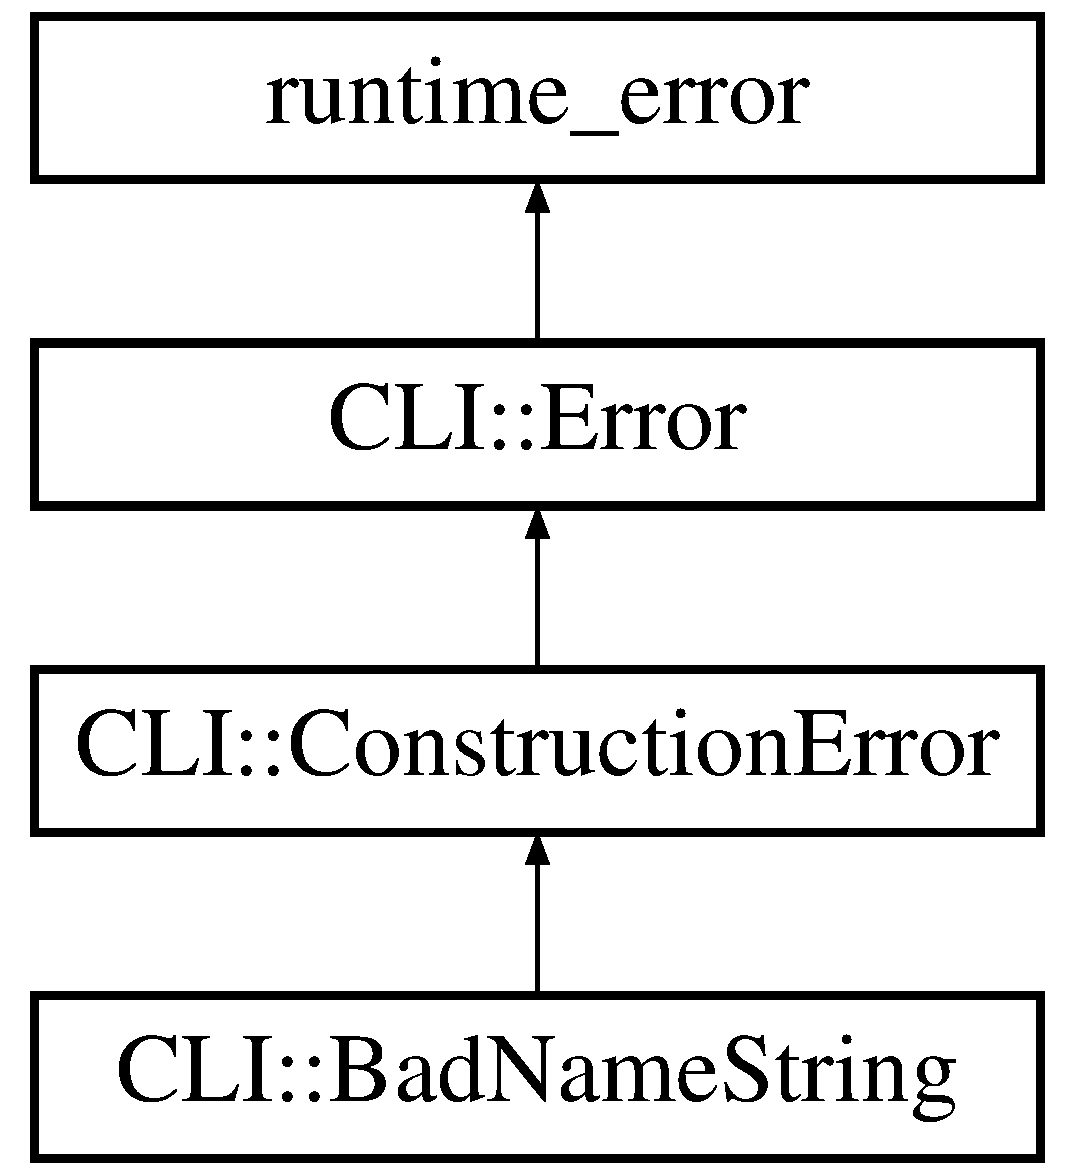
\includegraphics[height=4.000000cm]{struct_c_l_i_1_1_bad_name_string}
\end{center}
\end{figure}
\subsection*{Public Member Functions}
\begin{DoxyCompactItemize}
\item 
\mbox{\Hypertarget{struct_c_l_i_1_1_bad_name_string_ab1b309894dd5d3674a62c4fed7615fe9}\label{struct_c_l_i_1_1_bad_name_string_ab1b309894dd5d3674a62c4fed7615fe9}} 
{\bfseries Bad\+Name\+String} (std\+::string name)
\end{DoxyCompactItemize}
\subsection*{Additional Inherited Members}


\subsection{Detailed Description}
Thrown on construction of a bad name. 

The documentation for this struct was generated from the following file\+:\begin{DoxyCompactItemize}
\item 
/home/travis/build/henryiii/\+C\+L\+I11/include/\+C\+L\+I/Error.\+hpp\end{DoxyCompactItemize}

\hypertarget{struct_c_l_i_1_1_call_for_help}{}\section{C\+LI\+:\+:Call\+For\+Help Struct Reference}
\label{struct_c_l_i_1_1_call_for_help}\index{C\+L\+I\+::\+Call\+For\+Help@{C\+L\+I\+::\+Call\+For\+Help}}


-\/h or --help on command line  




{\ttfamily \#include $<$Error.\+hpp$>$}

Inheritance diagram for C\+LI\+:\+:Call\+For\+Help\+:\begin{figure}[H]
\begin{center}
\leavevmode
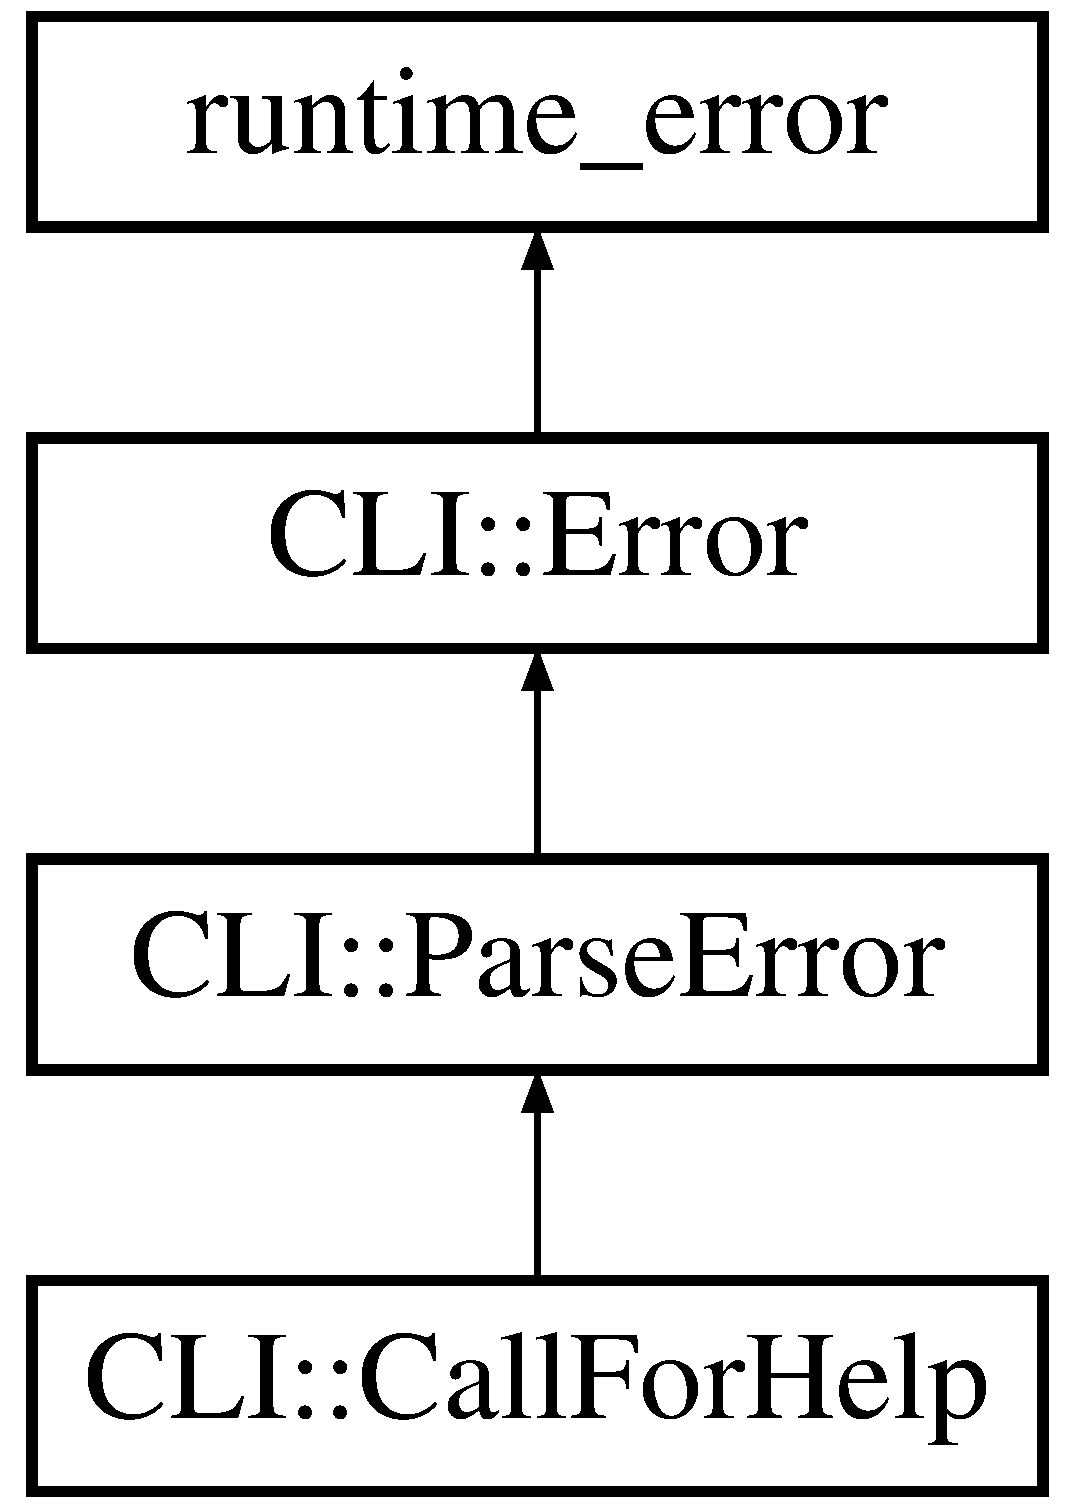
\includegraphics[height=4.000000cm]{struct_c_l_i_1_1_call_for_help}
\end{center}
\end{figure}
\subsection*{Additional Inherited Members}


\subsection{Detailed Description}
-\/h or --help on command line 

The documentation for this struct was generated from the following file\+:\begin{DoxyCompactItemize}
\item 
/home/travis/build/henryiii/\+C\+L\+I11/include/\+C\+L\+I/Error.\+hpp\end{DoxyCompactItemize}

\hypertarget{struct_c_l_i_1_1_construction_error}{}\section{C\+LI\+:\+:Construction\+Error Struct Reference}
\label{struct_c_l_i_1_1_construction_error}\index{C\+L\+I\+::\+Construction\+Error@{C\+L\+I\+::\+Construction\+Error}}


Construction errors (not in parsing)  




{\ttfamily \#include $<$Error.\+hpp$>$}

Inheritance diagram for C\+LI\+:\+:Construction\+Error\+:\begin{figure}[H]
\begin{center}
\leavevmode
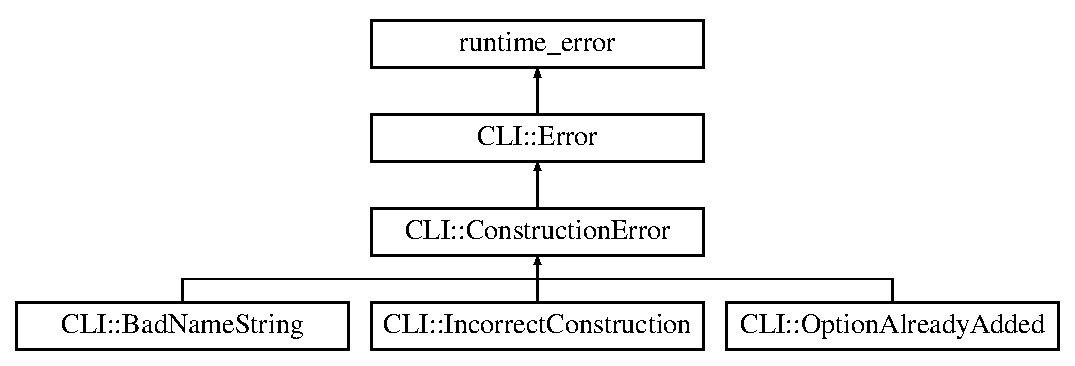
\includegraphics[height=4.000000cm]{struct_c_l_i_1_1_construction_error}
\end{center}
\end{figure}
\subsection*{Public Member Functions}
\begin{DoxyCompactItemize}
\item 
\mbox{\Hypertarget{struct_c_l_i_1_1_construction_error_a4172d6e095e73b537c22023b9ad2ae5a}\label{struct_c_l_i_1_1_construction_error_a4172d6e095e73b537c22023b9ad2ae5a}} 
{\bfseries Construction\+Error} (std\+::string parent, std\+::string name, int exit\+\_\+code=255, bool print\+\_\+help=true)
\end{DoxyCompactItemize}
\subsection*{Additional Inherited Members}


\subsection{Detailed Description}
Construction errors (not in parsing) 

The documentation for this struct was generated from the following file\+:\begin{DoxyCompactItemize}
\item 
/home/travis/build/henryiii/\+C\+L\+I11/include/\+C\+L\+I/Error.\+hpp\end{DoxyCompactItemize}

\hypertarget{struct_c_l_i_1_1_conversion_error}{}\section{C\+LI\+:\+:Conversion\+Error Struct Reference}
\label{struct_c_l_i_1_1_conversion_error}\index{C\+L\+I\+::\+Conversion\+Error@{C\+L\+I\+::\+Conversion\+Error}}


Thrown when conversion call back fails, such as when an int fails to coerse to a string.  




{\ttfamily \#include $<$Error.\+hpp$>$}

Inheritance diagram for C\+LI\+:\+:Conversion\+Error\+:\begin{figure}[H]
\begin{center}
\leavevmode
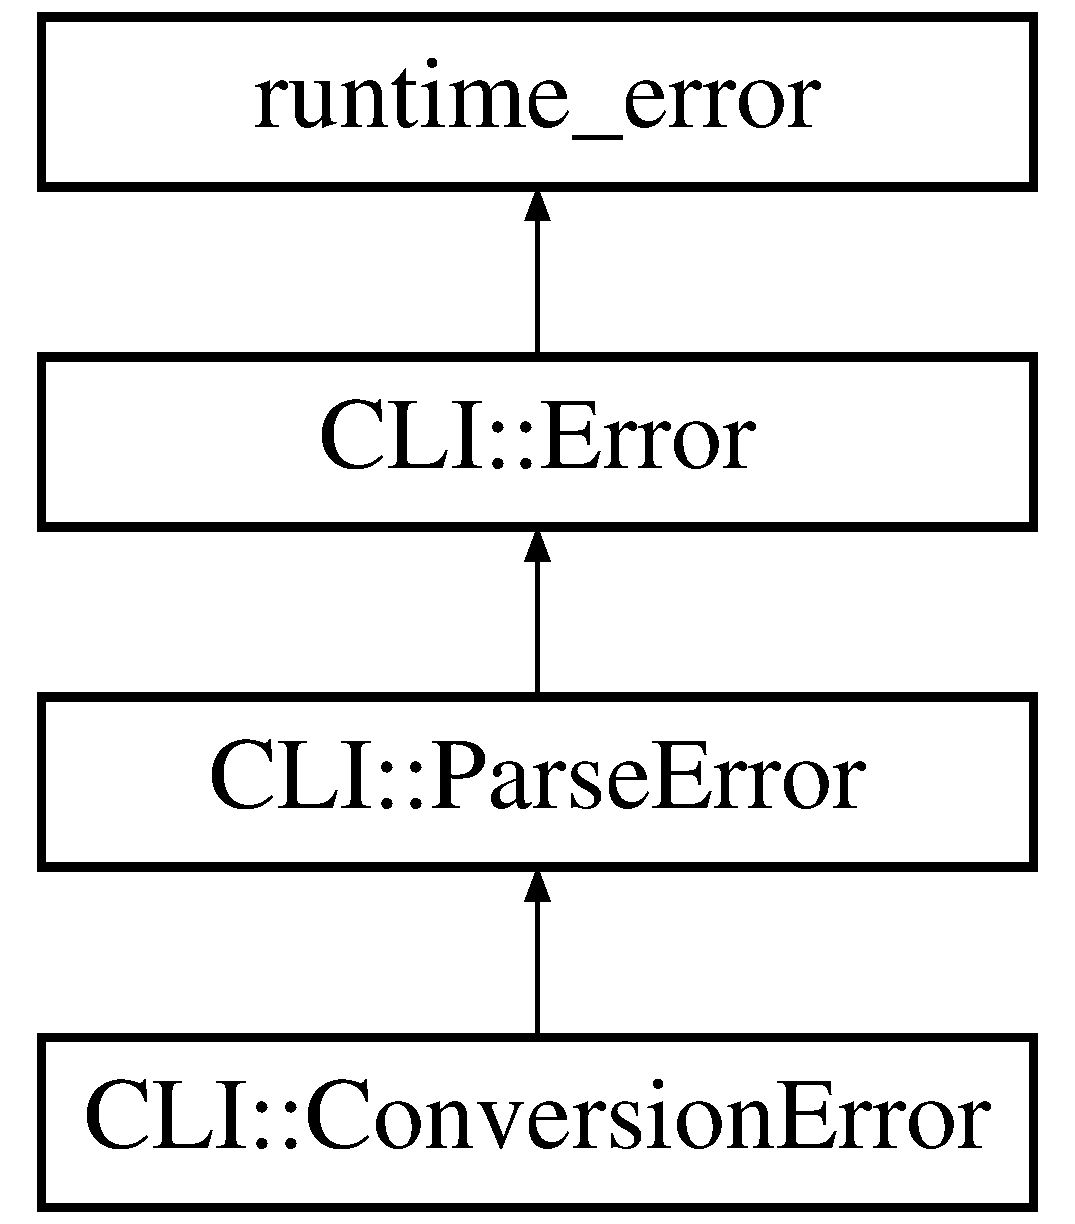
\includegraphics[height=4.000000cm]{struct_c_l_i_1_1_conversion_error}
\end{center}
\end{figure}
\subsection*{Public Member Functions}
\begin{DoxyCompactItemize}
\item 
\mbox{\Hypertarget{struct_c_l_i_1_1_conversion_error_a34cb19ea419b1730924966ca774788f0}\label{struct_c_l_i_1_1_conversion_error_a34cb19ea419b1730924966ca774788f0}} 
{\bfseries Conversion\+Error} (std\+::string name)
\end{DoxyCompactItemize}
\subsection*{Additional Inherited Members}


\subsection{Detailed Description}
Thrown when conversion call back fails, such as when an int fails to coerse to a string. 

The documentation for this struct was generated from the following file\+:\begin{DoxyCompactItemize}
\item 
/home/travis/build/henryiii/\+C\+L\+I11/include/\+C\+L\+I/Error.\+hpp\end{DoxyCompactItemize}

\hypertarget{struct_c_l_i_1_1_error}{}\section{C\+LI\+:\+:Error Struct Reference}
\label{struct_c_l_i_1_1_error}\index{C\+L\+I\+::\+Error@{C\+L\+I\+::\+Error}}


All errors derive from this one.  




{\ttfamily \#include $<$Error.\+hpp$>$}

Inheritance diagram for C\+LI\+:\+:Error\+:\begin{figure}[H]
\begin{center}
\leavevmode
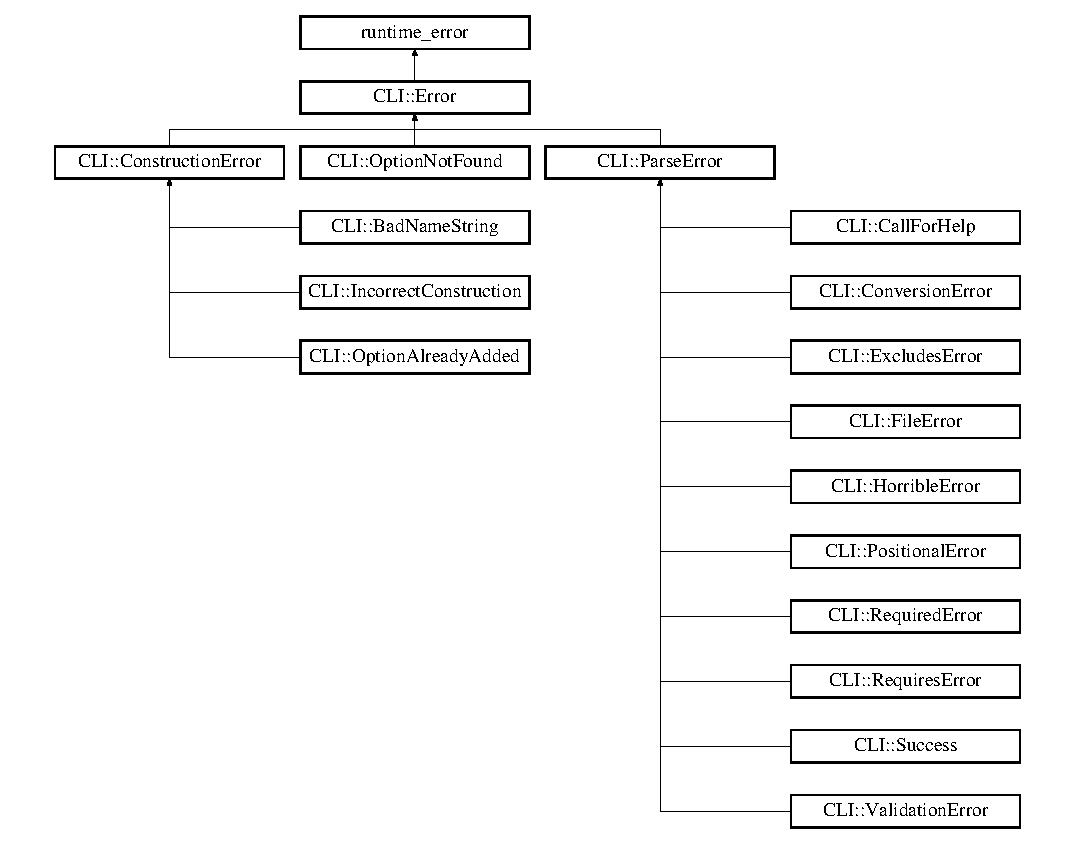
\includegraphics[height=10.898204cm]{struct_c_l_i_1_1_error}
\end{center}
\end{figure}
\subsection*{Public Member Functions}
\begin{DoxyCompactItemize}
\item 
\mbox{\Hypertarget{struct_c_l_i_1_1_error_a4a7d1df599d7b771bd46eb6f72221cc1}\label{struct_c_l_i_1_1_error_a4a7d1df599d7b771bd46eb6f72221cc1}} 
{\bfseries Error} (std\+::string parent, std\+::string name, int exit\+\_\+code=255, bool print\+\_\+help=true)
\end{DoxyCompactItemize}
\subsection*{Public Attributes}
\begin{DoxyCompactItemize}
\item 
\mbox{\Hypertarget{struct_c_l_i_1_1_error_ade74be0294e8a34fd8184b6c370b4b5e}\label{struct_c_l_i_1_1_error_ade74be0294e8a34fd8184b6c370b4b5e}} 
int {\bfseries exit\+\_\+code}
\item 
\mbox{\Hypertarget{struct_c_l_i_1_1_error_a6300b3fff4116be33fe52730b575ec34}\label{struct_c_l_i_1_1_error_a6300b3fff4116be33fe52730b575ec34}} 
bool {\bfseries print\+\_\+help}
\end{DoxyCompactItemize}


\subsection{Detailed Description}
All errors derive from this one. 

The documentation for this struct was generated from the following file\+:\begin{DoxyCompactItemize}
\item 
/home/travis/build/henryiii/\+C\+L\+I11/include/\+C\+L\+I/Error.\+hpp\end{DoxyCompactItemize}

\hypertarget{struct_c_l_i_1_1_excludes_error}{}\section{C\+LI\+:\+:Excludes\+Error Struct Reference}
\label{struct_c_l_i_1_1_excludes_error}\index{C\+L\+I\+::\+Excludes\+Error@{C\+L\+I\+::\+Excludes\+Error}}


Thrown when a exludes option is present.  




{\ttfamily \#include $<$Error.\+hpp$>$}

Inheritance diagram for C\+LI\+:\+:Excludes\+Error\+:\begin{figure}[H]
\begin{center}
\leavevmode
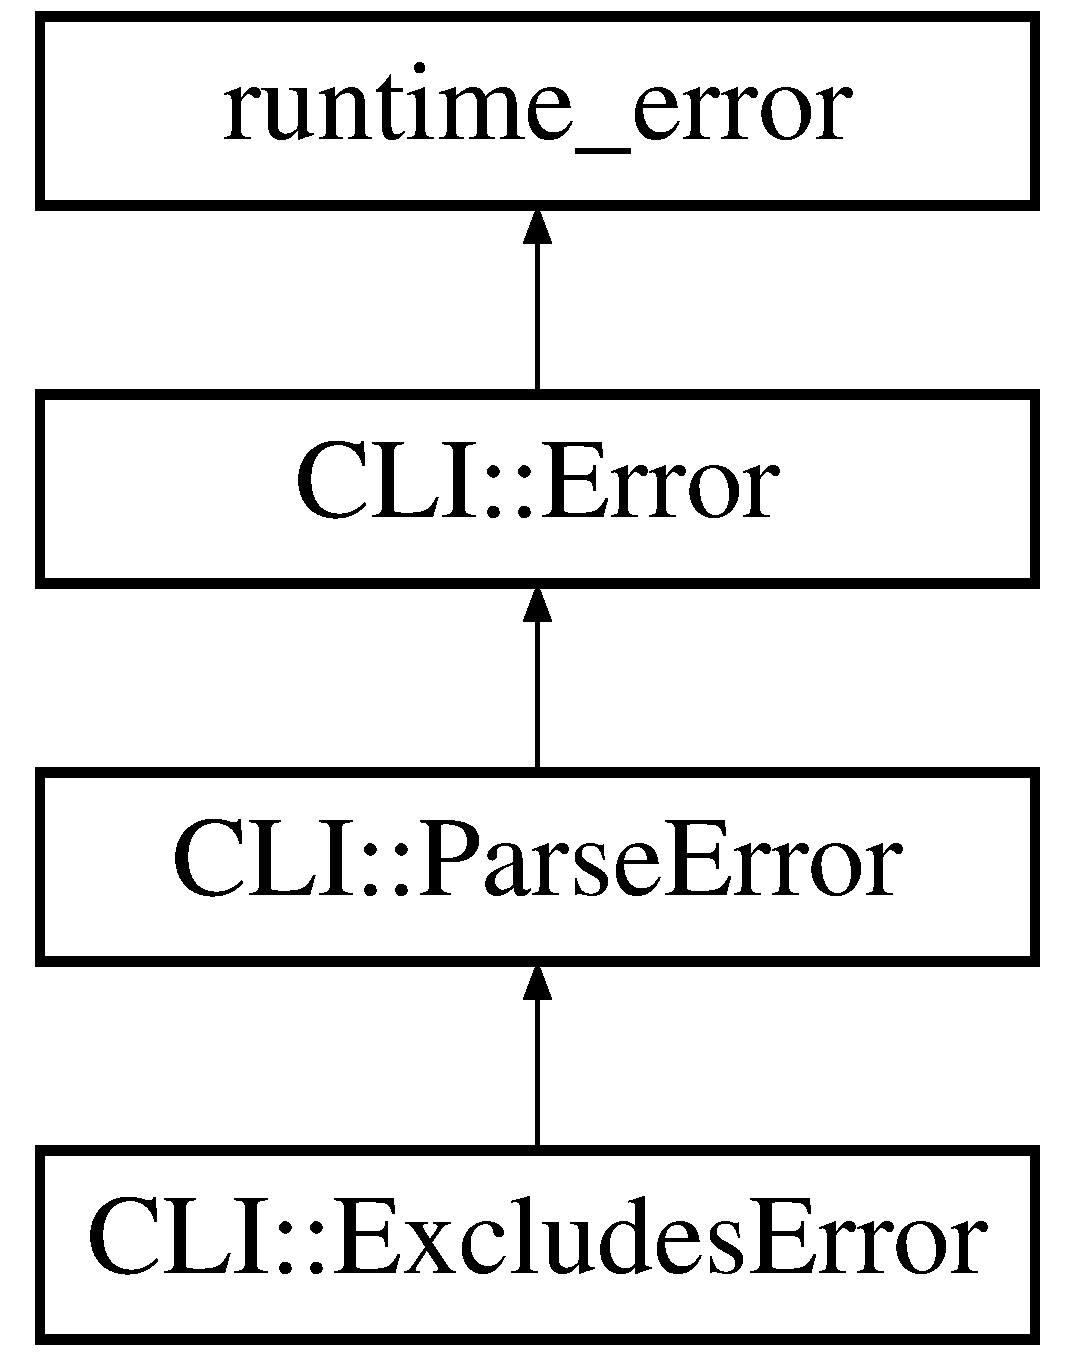
\includegraphics[height=4.000000cm]{struct_c_l_i_1_1_excludes_error}
\end{center}
\end{figure}
\subsection*{Public Member Functions}
\begin{DoxyCompactItemize}
\item 
\mbox{\Hypertarget{struct_c_l_i_1_1_excludes_error_ac019c598d7bd8bd6a370aaf05f0ddda2}\label{struct_c_l_i_1_1_excludes_error_ac019c598d7bd8bd6a370aaf05f0ddda2}} 
{\bfseries Excludes\+Error} (std\+::string name, std\+::string subname)
\end{DoxyCompactItemize}
\subsection*{Additional Inherited Members}


\subsection{Detailed Description}
Thrown when a exludes option is present. 

The documentation for this struct was generated from the following file\+:\begin{DoxyCompactItemize}
\item 
/home/travis/build/henryiii/\+C\+L\+I11/include/\+C\+L\+I/Error.\+hpp\end{DoxyCompactItemize}

\hypertarget{struct_c_l_i_1_1_file_error}{}\section{C\+LI\+:\+:File\+Error Struct Reference}
\label{struct_c_l_i_1_1_file_error}\index{C\+L\+I\+::\+File\+Error@{C\+L\+I\+::\+File\+Error}}


Thrown when parsing an I\+NI file and it is missing.  




{\ttfamily \#include $<$Error.\+hpp$>$}

Inheritance diagram for C\+LI\+:\+:File\+Error\+:\begin{figure}[H]
\begin{center}
\leavevmode
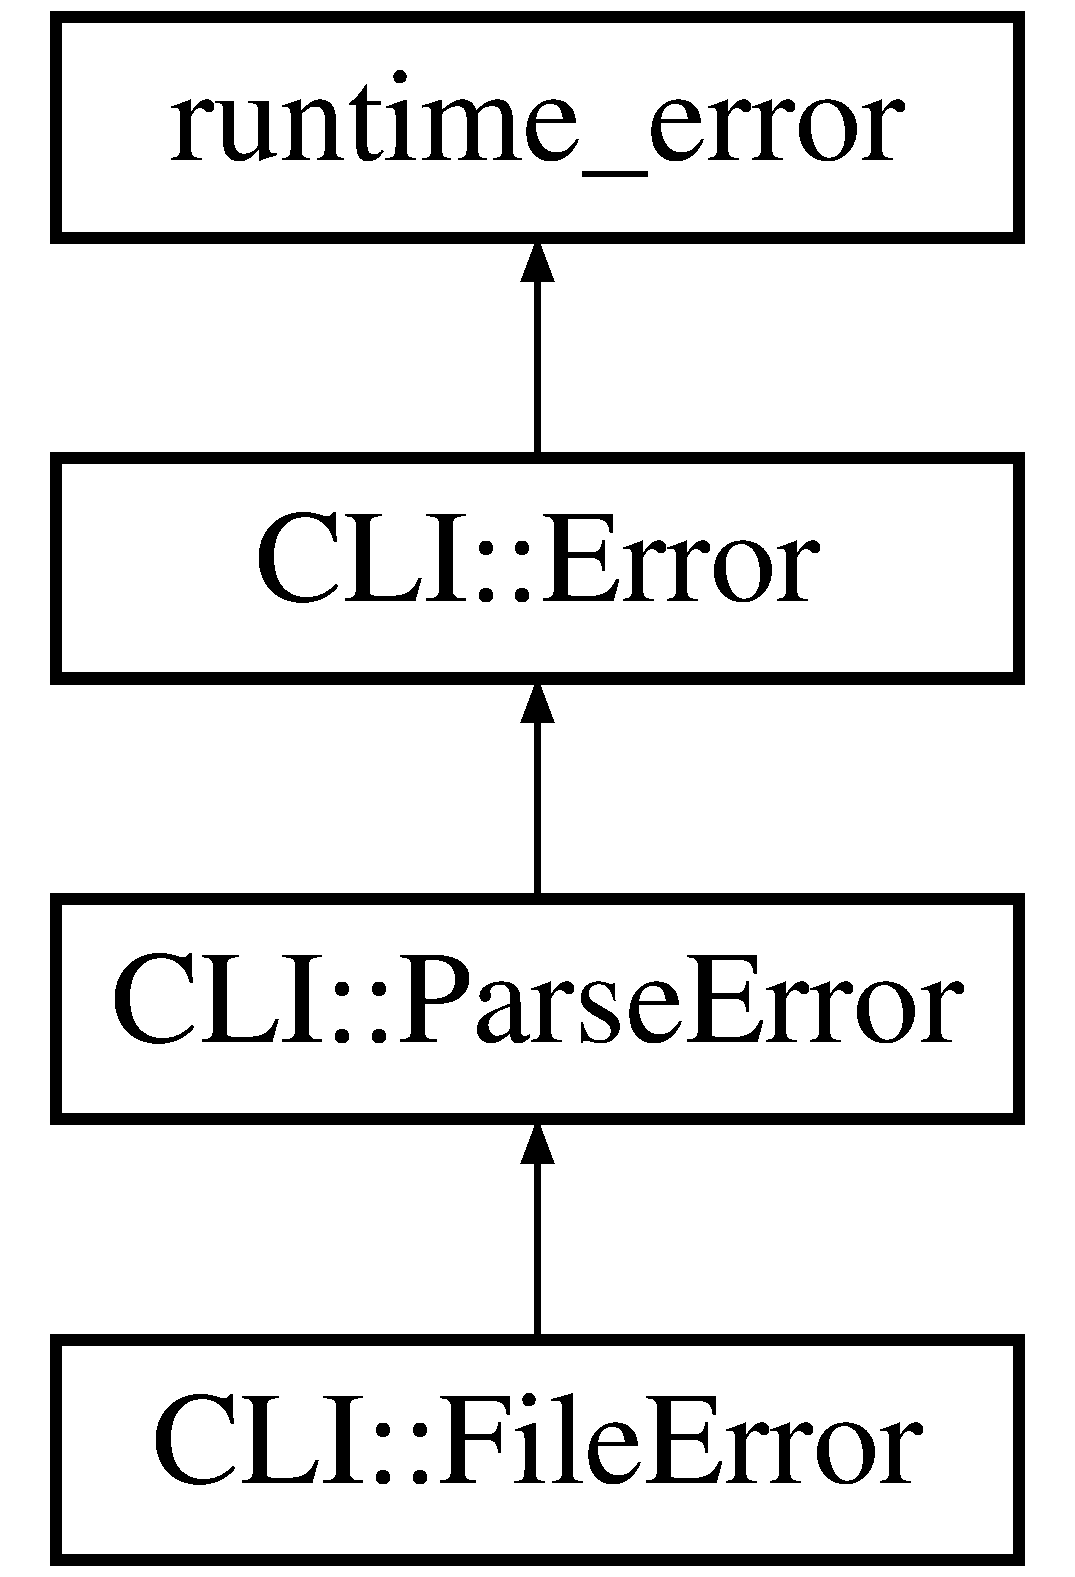
\includegraphics[height=4.000000cm]{struct_c_l_i_1_1_file_error}
\end{center}
\end{figure}
\subsection*{Public Member Functions}
\begin{DoxyCompactItemize}
\item 
\mbox{\Hypertarget{struct_c_l_i_1_1_file_error_a016a6b1162d93112a0446a0bc2afc68d}\label{struct_c_l_i_1_1_file_error_a016a6b1162d93112a0446a0bc2afc68d}} 
{\bfseries File\+Error} (std\+::string name)
\end{DoxyCompactItemize}
\subsection*{Additional Inherited Members}


\subsection{Detailed Description}
Thrown when parsing an I\+NI file and it is missing. 

The documentation for this struct was generated from the following file\+:\begin{DoxyCompactItemize}
\item 
/home/travis/build/henryiii/\+C\+L\+I11/include/\+C\+L\+I/Error.\+hpp\end{DoxyCompactItemize}

\hypertarget{struct_c_l_i_1_1_horrible_error}{}\section{C\+LI\+:\+:Horrible\+Error Struct Reference}
\label{struct_c_l_i_1_1_horrible_error}\index{C\+L\+I\+::\+Horrible\+Error@{C\+L\+I\+::\+Horrible\+Error}}


This is just a safety check to verify selection and parsing match.  




{\ttfamily \#include $<$Error.\+hpp$>$}

Inheritance diagram for C\+LI\+:\+:Horrible\+Error\+:\begin{figure}[H]
\begin{center}
\leavevmode
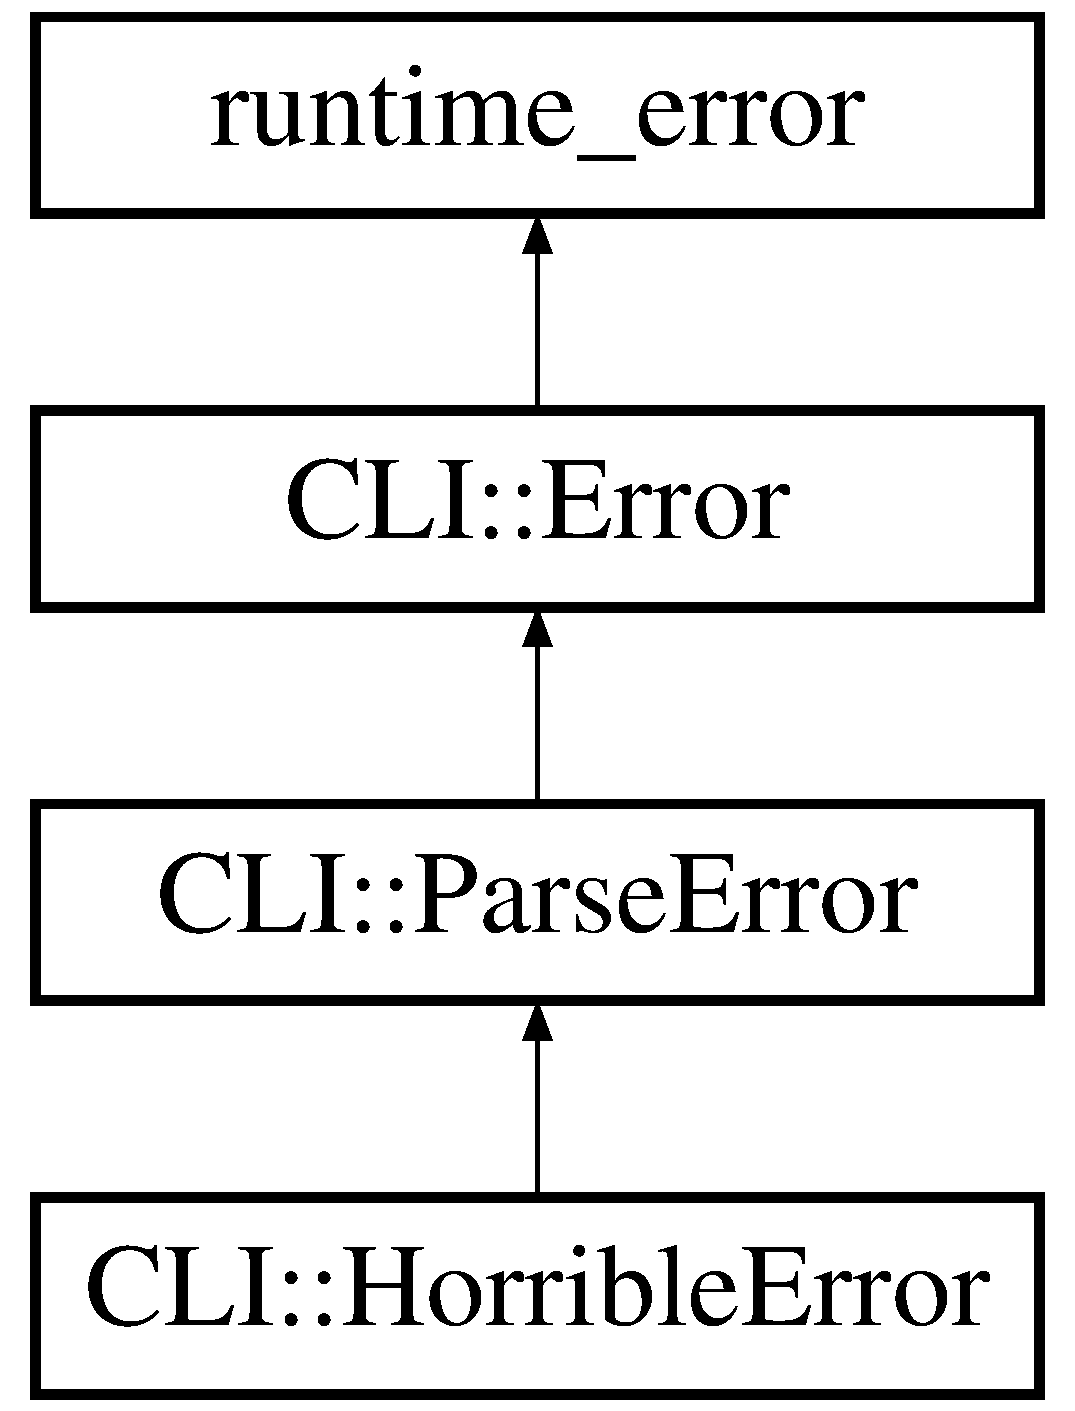
\includegraphics[height=4.000000cm]{struct_c_l_i_1_1_horrible_error}
\end{center}
\end{figure}
\subsection*{Public Member Functions}
\begin{DoxyCompactItemize}
\item 
\mbox{\Hypertarget{struct_c_l_i_1_1_horrible_error_a4883192c5b7e3f2a263caf24a09a86ec}\label{struct_c_l_i_1_1_horrible_error_a4883192c5b7e3f2a263caf24a09a86ec}} 
{\bfseries Horrible\+Error} (std\+::string name)
\end{DoxyCompactItemize}
\subsection*{Additional Inherited Members}


\subsection{Detailed Description}
This is just a safety check to verify selection and parsing match. 

The documentation for this struct was generated from the following file\+:\begin{DoxyCompactItemize}
\item 
/home/travis/build/henryiii/\+C\+L\+I11/include/\+C\+L\+I/Error.\+hpp\end{DoxyCompactItemize}

\hypertarget{struct_c_l_i_1_1_incorrect_construction}{}\section{C\+LI\+:\+:Incorrect\+Construction Struct Reference}
\label{struct_c_l_i_1_1_incorrect_construction}\index{C\+L\+I\+::\+Incorrect\+Construction@{C\+L\+I\+::\+Incorrect\+Construction}}


Thrown when an option is set to conflicting values (non-\/vector and multi args, for example)  




{\ttfamily \#include $<$Error.\+hpp$>$}

Inheritance diagram for C\+LI\+:\+:Incorrect\+Construction\+:\begin{figure}[H]
\begin{center}
\leavevmode
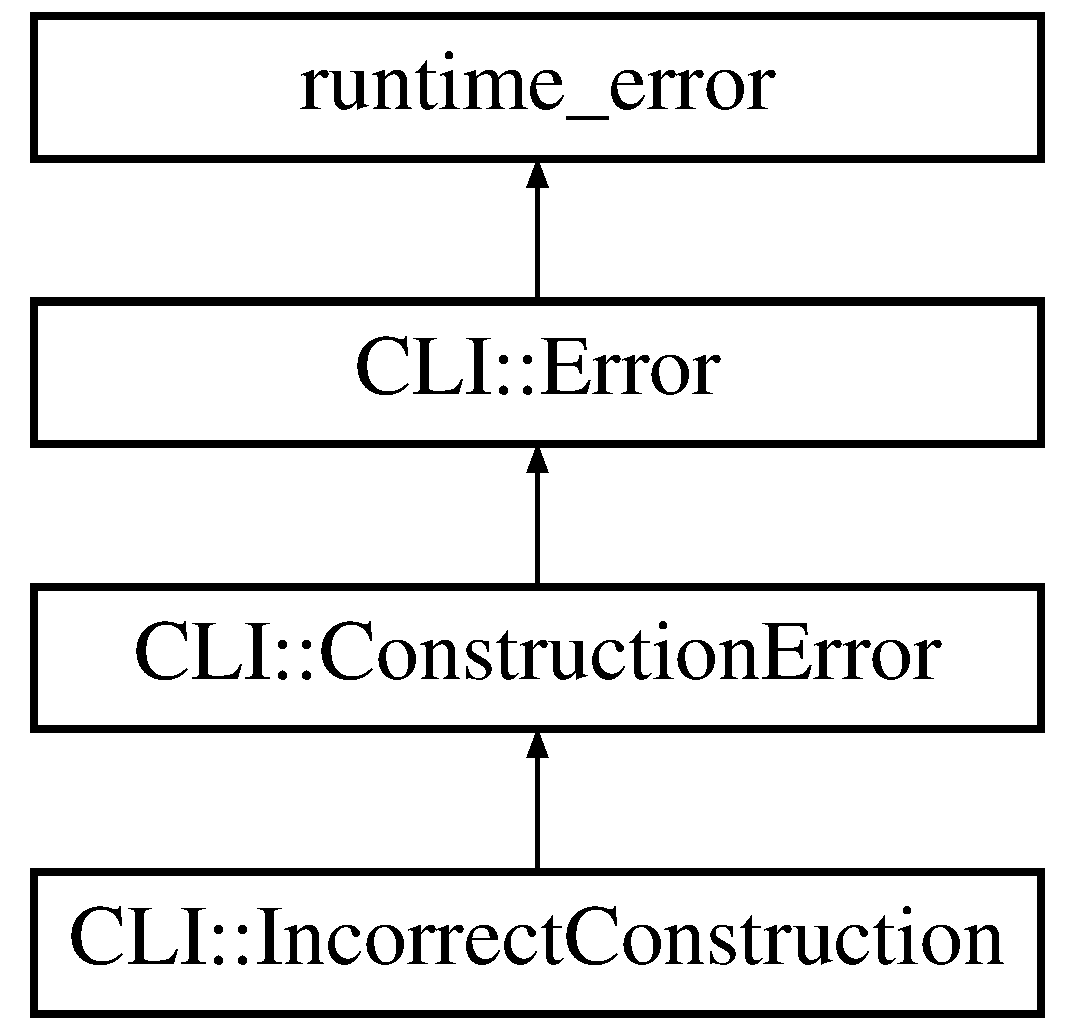
\includegraphics[height=4.000000cm]{struct_c_l_i_1_1_incorrect_construction}
\end{center}
\end{figure}
\subsection*{Public Member Functions}
\begin{DoxyCompactItemize}
\item 
\mbox{\Hypertarget{struct_c_l_i_1_1_incorrect_construction_a5d605f307996db7e763d02a5038377ff}\label{struct_c_l_i_1_1_incorrect_construction_a5d605f307996db7e763d02a5038377ff}} 
{\bfseries Incorrect\+Construction} (std\+::string name)
\end{DoxyCompactItemize}
\subsection*{Additional Inherited Members}


\subsection{Detailed Description}
Thrown when an option is set to conflicting values (non-\/vector and multi args, for example) 

The documentation for this struct was generated from the following file\+:\begin{DoxyCompactItemize}
\item 
/home/travis/build/henryiii/\+C\+L\+I11/include/\+C\+L\+I/Error.\+hpp\end{DoxyCompactItemize}

\hypertarget{struct_c_l_i_1_1is__bool}{}\section{C\+LI\+:\+:is\+\_\+bool$<$ T $>$ Struct Template Reference}
\label{struct_c_l_i_1_1is__bool}\index{C\+L\+I\+::is\+\_\+bool$<$ T $>$@{C\+L\+I\+::is\+\_\+bool$<$ T $>$}}
\subsection*{Static Public Attributes}
\begin{DoxyCompactItemize}
\item 
\mbox{\Hypertarget{struct_c_l_i_1_1is__bool_af31a1a454bf15231195d1a65c093f2f2}\label{struct_c_l_i_1_1is__bool_af31a1a454bf15231195d1a65c093f2f2}} 
static const bool {\bfseries value} = false
\end{DoxyCompactItemize}


The documentation for this struct was generated from the following file\+:\begin{DoxyCompactItemize}
\item 
/home/travis/build/henryiii/\+C\+L\+I11/include/\+C\+L\+I/Type\+Tools.\+hpp\end{DoxyCompactItemize}

\hypertarget{struct_c_l_i_1_1is__bool_3_01bool_01_4}{}\section{C\+LI\+:\+:is\+\_\+bool$<$ bool $>$ Struct Template Reference}
\label{struct_c_l_i_1_1is__bool_3_01bool_01_4}\index{C\+L\+I\+::is\+\_\+bool$<$ bool $>$@{C\+L\+I\+::is\+\_\+bool$<$ bool $>$}}
\subsection*{Static Public Attributes}
\begin{DoxyCompactItemize}
\item 
\mbox{\Hypertarget{struct_c_l_i_1_1is__bool_3_01bool_01_4_a54d8224c914b3935d8e827c7f1775a8e}\label{struct_c_l_i_1_1is__bool_3_01bool_01_4_a54d8224c914b3935d8e827c7f1775a8e}} 
static bool const {\bfseries value} = true
\end{DoxyCompactItemize}


The documentation for this struct was generated from the following file\+:\begin{DoxyCompactItemize}
\item 
/home/travis/build/henryiii/\+C\+L\+I11/include/\+C\+L\+I/Type\+Tools.\+hpp\end{DoxyCompactItemize}

\hypertarget{struct_c_l_i_1_1is__vector}{}\section{C\+LI\+:\+:is\+\_\+vector$<$ T $>$ Struct Template Reference}
\label{struct_c_l_i_1_1is__vector}\index{C\+L\+I\+::is\+\_\+vector$<$ T $>$@{C\+L\+I\+::is\+\_\+vector$<$ T $>$}}
\subsection*{Static Public Attributes}
\begin{DoxyCompactItemize}
\item 
\mbox{\Hypertarget{struct_c_l_i_1_1is__vector_a58b2d10b867ddfd6a71a70497fa20a19}\label{struct_c_l_i_1_1is__vector_a58b2d10b867ddfd6a71a70497fa20a19}} 
static const bool {\bfseries value} = false
\end{DoxyCompactItemize}


The documentation for this struct was generated from the following file\+:\begin{DoxyCompactItemize}
\item 
/home/travis/build/henryiii/\+C\+L\+I11/include/\+C\+L\+I/Type\+Tools.\+hpp\end{DoxyCompactItemize}

\hypertarget{struct_c_l_i_1_1is__vector_3_01std_1_1vector_3_01_t_00_01_a_01_4_01_4}{}\section{C\+LI\+:\+:is\+\_\+vector$<$ std\+:\+:vector$<$ T, A $>$ $>$ Struct Template Reference}
\label{struct_c_l_i_1_1is__vector_3_01std_1_1vector_3_01_t_00_01_a_01_4_01_4}\index{C\+L\+I\+::is\+\_\+vector$<$ std\+::vector$<$ T, A $>$ $>$@{C\+L\+I\+::is\+\_\+vector$<$ std\+::vector$<$ T, A $>$ $>$}}
\subsection*{Static Public Attributes}
\begin{DoxyCompactItemize}
\item 
\mbox{\Hypertarget{struct_c_l_i_1_1is__vector_3_01std_1_1vector_3_01_t_00_01_a_01_4_01_4_a3f57ff1f33bc35ee4d817047932307f0}\label{struct_c_l_i_1_1is__vector_3_01std_1_1vector_3_01_t_00_01_a_01_4_01_4_a3f57ff1f33bc35ee4d817047932307f0}} 
static bool const {\bfseries value} = true
\end{DoxyCompactItemize}


The documentation for this struct was generated from the following file\+:\begin{DoxyCompactItemize}
\item 
/home/travis/build/henryiii/\+C\+L\+I11/include/\+C\+L\+I/Type\+Tools.\+hpp\end{DoxyCompactItemize}

\hypertarget{class_c_l_i_1_1_option}{}\section{C\+LI\+:\+:Option Class Reference}
\label{class_c_l_i_1_1_option}\index{C\+L\+I\+::\+Option@{C\+L\+I\+::\+Option}}
\subsection*{Public Member Functions}
\begin{DoxyCompactItemize}
\item 
\mbox{\Hypertarget{class_c_l_i_1_1_option_a2ea1f937d3537b3f06f6fe723ab271c4}\label{class_c_l_i_1_1_option_a2ea1f937d3537b3f06f6fe723ab271c4}} 
{\bfseries Option} (std\+::string name, std\+::string description=\char`\"{}\char`\"{}, std\+::function$<$ bool(results\+\_\+t)$>$ callback=\mbox{[}$\,$\mbox{]}(results\+\_\+t)\{return true;\}, bool \+\_\+default=true)
\item 
\mbox{\Hypertarget{class_c_l_i_1_1_option_ab73e846fb3a78ac7eff8b6cd6afb24a1}\label{class_c_l_i_1_1_option_ab73e846fb3a78ac7eff8b6cd6afb24a1}} 
{\bfseries operator bool} () const
\item 
\mbox{\Hypertarget{class_c_l_i_1_1_option_abbd36aaff5cdca8b10346bafed51da39}\label{class_c_l_i_1_1_option_abbd36aaff5cdca8b10346bafed51da39}} 
void \hyperlink{class_c_l_i_1_1_option_abbd36aaff5cdca8b10346bafed51da39}{clear} ()
\begin{DoxyCompactList}\small\item\em Clear the parsed results (mostly for testing) \end{DoxyCompactList}\item 
\mbox{\Hypertarget{class_c_l_i_1_1_option_a950395187e95aec210928b36e90621bb}\label{class_c_l_i_1_1_option_a950395187e95aec210928b36e90621bb}} 
\hyperlink{class_c_l_i_1_1_option}{Option} $\ast$ \hyperlink{class_c_l_i_1_1_option_a950395187e95aec210928b36e90621bb}{required} (bool value=true)
\begin{DoxyCompactList}\small\item\em Set the option as required. \end{DoxyCompactList}\item 
\mbox{\Hypertarget{class_c_l_i_1_1_option_a04d6a400482ecaa08cc5b3a93f0ca93c}\label{class_c_l_i_1_1_option_a04d6a400482ecaa08cc5b3a93f0ca93c}} 
\hyperlink{class_c_l_i_1_1_option}{Option} $\ast$ \hyperlink{class_c_l_i_1_1_option_a04d6a400482ecaa08cc5b3a93f0ca93c}{mandatory} (bool value=true)
\begin{DoxyCompactList}\small\item\em Support Plubmum term. \end{DoxyCompactList}\item 
\mbox{\Hypertarget{class_c_l_i_1_1_option_a1b1aaa271902bca28a2c526d015a93c1}\label{class_c_l_i_1_1_option_a1b1aaa271902bca28a2c526d015a93c1}} 
bool \hyperlink{class_c_l_i_1_1_option_a1b1aaa271902bca28a2c526d015a93c1}{get\+\_\+required} () const
\begin{DoxyCompactList}\small\item\em True if this is a required option. \end{DoxyCompactList}\item 
\mbox{\Hypertarget{class_c_l_i_1_1_option_af75c26433baa09c7c762bfb9eb466215}\label{class_c_l_i_1_1_option_af75c26433baa09c7c762bfb9eb466215}} 
\hyperlink{class_c_l_i_1_1_option}{Option} $\ast$ \hyperlink{class_c_l_i_1_1_option_af75c26433baa09c7c762bfb9eb466215}{expected} (int value)
\begin{DoxyCompactList}\small\item\em Set the number of expected arguments (Flags bypass this) \end{DoxyCompactList}\item 
\mbox{\Hypertarget{class_c_l_i_1_1_option_a307543e6e4ddeb6e4ea00438b5b10be3}\label{class_c_l_i_1_1_option_a307543e6e4ddeb6e4ea00438b5b10be3}} 
int \hyperlink{class_c_l_i_1_1_option_a307543e6e4ddeb6e4ea00438b5b10be3}{get\+\_\+expected} () const
\begin{DoxyCompactList}\small\item\em The number of arguments the option expects. \end{DoxyCompactList}\item 
\mbox{\Hypertarget{class_c_l_i_1_1_option_a26527442a386c8ccc369069c00062398}\label{class_c_l_i_1_1_option_a26527442a386c8ccc369069c00062398}} 
int \hyperlink{class_c_l_i_1_1_option_a26527442a386c8ccc369069c00062398}{get\+\_\+default} () const
\begin{DoxyCompactList}\small\item\em True if this has a default value. \end{DoxyCompactList}\item 
\mbox{\Hypertarget{class_c_l_i_1_1_option_acab7033604b49e314d290b01adea690d}\label{class_c_l_i_1_1_option_acab7033604b49e314d290b01adea690d}} 
bool \hyperlink{class_c_l_i_1_1_option_acab7033604b49e314d290b01adea690d}{get\+\_\+positional} () const
\begin{DoxyCompactList}\small\item\em True if the argument can be given directly. \end{DoxyCompactList}\item 
\mbox{\Hypertarget{class_c_l_i_1_1_option_a94cc5149d388be946c449e8ee61cd034}\label{class_c_l_i_1_1_option_a94cc5149d388be946c449e8ee61cd034}} 
bool \hyperlink{class_c_l_i_1_1_option_a94cc5149d388be946c449e8ee61cd034}{nonpositional} () const
\begin{DoxyCompactList}\small\item\em True if option has at least one non-\/positional name. \end{DoxyCompactList}\item 
\mbox{\Hypertarget{class_c_l_i_1_1_option_a6770984498050b33659ce0c14b8f4696}\label{class_c_l_i_1_1_option_a6770984498050b33659ce0c14b8f4696}} 
bool \hyperlink{class_c_l_i_1_1_option_a6770984498050b33659ce0c14b8f4696}{has\+\_\+description} () const
\begin{DoxyCompactList}\small\item\em True if option has description. \end{DoxyCompactList}\item 
\mbox{\Hypertarget{class_c_l_i_1_1_option_a4dbdf09db906dda9417c80ee1676e0af}\label{class_c_l_i_1_1_option_a4dbdf09db906dda9417c80ee1676e0af}} 
\hyperlink{class_c_l_i_1_1_option}{Option} $\ast$ \hyperlink{class_c_l_i_1_1_option_a4dbdf09db906dda9417c80ee1676e0af}{check} (std\+::function$<$ bool(std\+::string)$>$ validator)
\begin{DoxyCompactList}\small\item\em Adds a validator. \end{DoxyCompactList}\item 
\mbox{\Hypertarget{class_c_l_i_1_1_option_aab4b629426409424e9d852170ee18796}\label{class_c_l_i_1_1_option_aab4b629426409424e9d852170ee18796}} 
\hyperlink{class_c_l_i_1_1_option}{Option} $\ast$ \hyperlink{class_c_l_i_1_1_option_aab4b629426409424e9d852170ee18796}{group} (std\+::string name)
\begin{DoxyCompactList}\small\item\em Changes the group membership. \end{DoxyCompactList}\item 
\mbox{\Hypertarget{class_c_l_i_1_1_option_a5f6adbac10f12a3865e94d6ad59f2a83}\label{class_c_l_i_1_1_option_a5f6adbac10f12a3865e94d6ad59f2a83}} 
const std\+::string \& \hyperlink{class_c_l_i_1_1_option_a5f6adbac10f12a3865e94d6ad59f2a83}{get\+\_\+group} () const
\begin{DoxyCompactList}\small\item\em Get the group of this option. \end{DoxyCompactList}\item 
\mbox{\Hypertarget{class_c_l_i_1_1_option_ad79474a3c1cc8a73b12f80c6e31ee3af}\label{class_c_l_i_1_1_option_ad79474a3c1cc8a73b12f80c6e31ee3af}} 
const std\+::string \& \hyperlink{class_c_l_i_1_1_option_ad79474a3c1cc8a73b12f80c6e31ee3af}{get\+\_\+description} () const
\begin{DoxyCompactList}\small\item\em Get the description. \end{DoxyCompactList}\item 
\mbox{\Hypertarget{class_c_l_i_1_1_option_abee0e47f0df529a1d0b2cc9ed2ca33d9}\label{class_c_l_i_1_1_option_abee0e47f0df529a1d0b2cc9ed2ca33d9}} 
\hyperlink{class_c_l_i_1_1_option}{Option} $\ast$ \hyperlink{class_c_l_i_1_1_option_abee0e47f0df529a1d0b2cc9ed2ca33d9}{requires} (\hyperlink{class_c_l_i_1_1_option}{Option} $\ast$opt)
\begin{DoxyCompactList}\small\item\em Sets required options. \end{DoxyCompactList}\item 
\mbox{\Hypertarget{class_c_l_i_1_1_option_a6edf22002aebe6e0ac69c61283be4ec5}\label{class_c_l_i_1_1_option_a6edf22002aebe6e0ac69c61283be4ec5}} 
{\footnotesize template$<$typename... A\+RG$>$ }\\\hyperlink{class_c_l_i_1_1_option}{Option} $\ast$ \hyperlink{class_c_l_i_1_1_option_a6edf22002aebe6e0ac69c61283be4ec5}{requires} (\hyperlink{class_c_l_i_1_1_option}{Option} $\ast$opt, \hyperlink{class_c_l_i_1_1_option}{Option} $\ast$opt1, A\+R\+G... args)
\begin{DoxyCompactList}\small\item\em Any number supported. \end{DoxyCompactList}\item 
\mbox{\Hypertarget{class_c_l_i_1_1_option_a9597b8271ebc4ad41c2e86f31834a1a3}\label{class_c_l_i_1_1_option_a9597b8271ebc4ad41c2e86f31834a1a3}} 
\hyperlink{class_c_l_i_1_1_option}{Option} $\ast$ \hyperlink{class_c_l_i_1_1_option_a9597b8271ebc4ad41c2e86f31834a1a3}{excludes} (\hyperlink{class_c_l_i_1_1_option}{Option} $\ast$opt)
\begin{DoxyCompactList}\small\item\em Sets excluded options. \end{DoxyCompactList}\item 
\mbox{\Hypertarget{class_c_l_i_1_1_option_a1af39fb37a32be1b95f9fe582744d471}\label{class_c_l_i_1_1_option_a1af39fb37a32be1b95f9fe582744d471}} 
{\footnotesize template$<$typename... A\+RG$>$ }\\\hyperlink{class_c_l_i_1_1_option}{Option} $\ast$ \hyperlink{class_c_l_i_1_1_option_a1af39fb37a32be1b95f9fe582744d471}{excludes} (\hyperlink{class_c_l_i_1_1_option}{Option} $\ast$opt, \hyperlink{class_c_l_i_1_1_option}{Option} $\ast$opt1, A\+R\+G... args)
\begin{DoxyCompactList}\small\item\em Any number supported. \end{DoxyCompactList}\item 
\mbox{\Hypertarget{class_c_l_i_1_1_option_aa1969c5f5a525910d761756a6d8e63a8}\label{class_c_l_i_1_1_option_aa1969c5f5a525910d761756a6d8e63a8}} 
\hyperlink{class_c_l_i_1_1_option}{Option} $\ast$ \hyperlink{class_c_l_i_1_1_option_aa1969c5f5a525910d761756a6d8e63a8}{envname} (std\+::string name)
\begin{DoxyCompactList}\small\item\em Sets environment variable to read if no option given. \end{DoxyCompactList}\item 
\mbox{\Hypertarget{class_c_l_i_1_1_option_a4b4efb7ea6c264b3dc09f5022121a9fe}\label{class_c_l_i_1_1_option_a4b4efb7ea6c264b3dc09f5022121a9fe}} 
std\+::string \hyperlink{class_c_l_i_1_1_option_a4b4efb7ea6c264b3dc09f5022121a9fe}{help\+\_\+positional} () const
\begin{DoxyCompactList}\small\item\em The name and any extras needed for positionals. \end{DoxyCompactList}\item 
\mbox{\Hypertarget{class_c_l_i_1_1_option_a5b887cdb58ce7b840417e41567eb507b}\label{class_c_l_i_1_1_option_a5b887cdb58ce7b840417e41567eb507b}} 
std\+::string {\bfseries get\+\_\+pname} () const
\item 
\mbox{\Hypertarget{class_c_l_i_1_1_option_adb852929843300c4b48de5556ceea1b1}\label{class_c_l_i_1_1_option_adb852929843300c4b48de5556ceea1b1}} 
void \hyperlink{class_c_l_i_1_1_option_adb852929843300c4b48de5556ceea1b1}{run\+\_\+callback} () const
\begin{DoxyCompactList}\small\item\em Process the callback. \end{DoxyCompactList}\item 
\mbox{\Hypertarget{class_c_l_i_1_1_option_ae72ff0b89bebb2987d548c186c577e50}\label{class_c_l_i_1_1_option_ae72ff0b89bebb2987d548c186c577e50}} 
bool \hyperlink{class_c_l_i_1_1_option_ae72ff0b89bebb2987d548c186c577e50}{operator==} (const \hyperlink{class_c_l_i_1_1_option}{Option} \&other) const
\begin{DoxyCompactList}\small\item\em If options share any of the same names, they are equal (not counting positional) \end{DoxyCompactList}\item 
\mbox{\Hypertarget{class_c_l_i_1_1_option_a21524238e17fd0367f4a3528665e7816}\label{class_c_l_i_1_1_option_a21524238e17fd0367f4a3528665e7816}} 
std\+::string \hyperlink{class_c_l_i_1_1_option_a21524238e17fd0367f4a3528665e7816}{get\+\_\+name} (bool opt\+\_\+only=false) const
\begin{DoxyCompactList}\small\item\em Gets a , sep list of names. Does not include the positional name if opt\+\_\+only=true. \end{DoxyCompactList}\item 
\mbox{\Hypertarget{class_c_l_i_1_1_option_af457a9a493f06f212cad9f854b281200}\label{class_c_l_i_1_1_option_af457a9a493f06f212cad9f854b281200}} 
bool \hyperlink{class_c_l_i_1_1_option_af457a9a493f06f212cad9f854b281200}{check\+\_\+name} (std\+::string name) const
\begin{DoxyCompactList}\small\item\em Check a name. Requires \char`\"{}-\/\char`\"{} or \char`\"{}-\/-\/\char`\"{} for short / long, supports positional name. \end{DoxyCompactList}\item 
\mbox{\Hypertarget{class_c_l_i_1_1_option_adc89601cb96badc8299eebac5f158160}\label{class_c_l_i_1_1_option_adc89601cb96badc8299eebac5f158160}} 
bool \hyperlink{class_c_l_i_1_1_option_adc89601cb96badc8299eebac5f158160}{check\+\_\+sname} (const std\+::string \&name) const
\begin{DoxyCompactList}\small\item\em Requires \char`\"{}-\/\char`\"{} to be removed from string. \end{DoxyCompactList}\item 
\mbox{\Hypertarget{class_c_l_i_1_1_option_aab0fc59aaa0e04b9bfe1495702ba679e}\label{class_c_l_i_1_1_option_aab0fc59aaa0e04b9bfe1495702ba679e}} 
bool \hyperlink{class_c_l_i_1_1_option_aab0fc59aaa0e04b9bfe1495702ba679e}{check\+\_\+lname} (const std\+::string \&name) const
\begin{DoxyCompactList}\small\item\em Requires \char`\"{}-\/-\/\char`\"{} to be removed from string. \end{DoxyCompactList}\item 
\mbox{\Hypertarget{class_c_l_i_1_1_option_a8f6617a899c47c04eb63521116668c9b}\label{class_c_l_i_1_1_option_a8f6617a899c47c04eb63521116668c9b}} 
void \hyperlink{class_c_l_i_1_1_option_a8f6617a899c47c04eb63521116668c9b}{add\+\_\+result} (int r, std\+::string s)
\begin{DoxyCompactList}\small\item\em Puts a result at position r. \end{DoxyCompactList}\item 
\mbox{\Hypertarget{class_c_l_i_1_1_option_a72c906e471759afcbcf52e04288e44ab}\label{class_c_l_i_1_1_option_a72c906e471759afcbcf52e04288e44ab}} 
int \hyperlink{class_c_l_i_1_1_option_a72c906e471759afcbcf52e04288e44ab}{get\+\_\+new} ()
\begin{DoxyCompactList}\small\item\em Starts a new results vector (used for r in add\+\_\+result) \end{DoxyCompactList}\item 
\mbox{\Hypertarget{class_c_l_i_1_1_option_ac1f93311a6577359953e54a2e575ae71}\label{class_c_l_i_1_1_option_ac1f93311a6577359953e54a2e575ae71}} 
int \hyperlink{class_c_l_i_1_1_option_ac1f93311a6577359953e54a2e575ae71}{count} () const
\begin{DoxyCompactList}\small\item\em Count the total number of times an option was passed. \end{DoxyCompactList}\item 
\mbox{\Hypertarget{class_c_l_i_1_1_option_a04678f59beb4efd6f6641f7684410521}\label{class_c_l_i_1_1_option_a04678f59beb4efd6f6641f7684410521}} 
std\+::string \hyperlink{class_c_l_i_1_1_option_a04678f59beb4efd6f6641f7684410521}{help\+\_\+name} () const
\begin{DoxyCompactList}\small\item\em The first half of the help print, name plus default, etc. \end{DoxyCompactList}\item 
\mbox{\Hypertarget{class_c_l_i_1_1_option_adc163181d02633344838b04191624306}\label{class_c_l_i_1_1_option_adc163181d02633344838b04191624306}} 
std\+::string \hyperlink{class_c_l_i_1_1_option_adc163181d02633344838b04191624306}{help\+\_\+pname} () const
\begin{DoxyCompactList}\small\item\em pname with type info \end{DoxyCompactList}\item 
\mbox{\Hypertarget{class_c_l_i_1_1_option_a29b64a9a6ed7bbc5966801b221018aa9}\label{class_c_l_i_1_1_option_a29b64a9a6ed7bbc5966801b221018aa9}} 
std\+::string \hyperlink{class_c_l_i_1_1_option_a29b64a9a6ed7bbc5966801b221018aa9}{\+\_\+help\+\_\+aftername} () const
\begin{DoxyCompactList}\small\item\em This is the part after the name is printed but before the description. \end{DoxyCompactList}\item 
\mbox{\Hypertarget{class_c_l_i_1_1_option_abf59d86491287a29f76aead3818a2770}\label{class_c_l_i_1_1_option_abf59d86491287a29f76aead3818a2770}} 
std\+::vector$<$ std\+::string $>$ \hyperlink{class_c_l_i_1_1_option_abf59d86491287a29f76aead3818a2770}{flatten\+\_\+results} () const
\begin{DoxyCompactList}\small\item\em Produce a flattened vector of results, vs. a vector of vectors. \end{DoxyCompactList}\end{DoxyCompactItemize}
\subsection*{Protected Attributes}
\begin{DoxyCompactItemize}
\item 
\mbox{\Hypertarget{class_c_l_i_1_1_option_ac28157805c3d7e13dc5636d01c3d4913}\label{class_c_l_i_1_1_option_ac28157805c3d7e13dc5636d01c3d4913}} 
std\+::vector$<$ std\+::string $>$ {\bfseries snames}
\item 
\mbox{\Hypertarget{class_c_l_i_1_1_option_a93808c6deea5e76a285122d97411fb21}\label{class_c_l_i_1_1_option_a93808c6deea5e76a285122d97411fb21}} 
std\+::vector$<$ std\+::string $>$ {\bfseries lnames}
\item 
\mbox{\Hypertarget{class_c_l_i_1_1_option_add0264f8eb6029868704f9127b1d5dde}\label{class_c_l_i_1_1_option_add0264f8eb6029868704f9127b1d5dde}} 
std\+::string {\bfseries pname}
\item 
\mbox{\Hypertarget{class_c_l_i_1_1_option_a09ff254da5e446741cc1267fd988fc12}\label{class_c_l_i_1_1_option_a09ff254da5e446741cc1267fd988fc12}} 
std\+::string {\bfseries description}
\item 
\mbox{\Hypertarget{class_c_l_i_1_1_option_ad7e58b3981990eca42fc3c5631157d64}\label{class_c_l_i_1_1_option_ad7e58b3981990eca42fc3c5631157d64}} 
callback\+\_\+t {\bfseries callback}
\item 
\mbox{\Hypertarget{class_c_l_i_1_1_option_a8ceb8093d3379a4570bf022119e6cc00}\label{class_c_l_i_1_1_option_a8ceb8093d3379a4570bf022119e6cc00}} 
std\+::string {\bfseries defaultval}
\item 
\mbox{\Hypertarget{class_c_l_i_1_1_option_afeef9734a60b2f0f244ba06ac6add35d}\label{class_c_l_i_1_1_option_afeef9734a60b2f0f244ba06ac6add35d}} 
std\+::string {\bfseries typeval}
\item 
\mbox{\Hypertarget{class_c_l_i_1_1_option_ab9ac4458f54b5f815cb6e33b9b8b3e79}\label{class_c_l_i_1_1_option_ab9ac4458f54b5f815cb6e33b9b8b3e79}} 
std\+::string {\bfseries \+\_\+group} \{\char`\"{}Options\char`\"{}\}
\item 
\mbox{\Hypertarget{class_c_l_i_1_1_option_a8f9325c2b17a30159d1fb7499655f7fd}\label{class_c_l_i_1_1_option_a8f9325c2b17a30159d1fb7499655f7fd}} 
bool {\bfseries \+\_\+default} \{false\}
\item 
\mbox{\Hypertarget{class_c_l_i_1_1_option_a0223f2dffff5cabced014d33157d417f}\label{class_c_l_i_1_1_option_a0223f2dffff5cabced014d33157d417f}} 
bool {\bfseries \+\_\+required} \{false\}
\item 
\mbox{\Hypertarget{class_c_l_i_1_1_option_a5ae06c4d699b1d0dda2b02f1b8a10471}\label{class_c_l_i_1_1_option_a5ae06c4d699b1d0dda2b02f1b8a10471}} 
int {\bfseries \+\_\+expected} \{1\}
\item 
\mbox{\Hypertarget{class_c_l_i_1_1_option_a2ea97d9c465a9f513a609798aad1efde}\label{class_c_l_i_1_1_option_a2ea97d9c465a9f513a609798aad1efde}} 
bool {\bfseries allow\+\_\+vector} \{false\}
\item 
\mbox{\Hypertarget{class_c_l_i_1_1_option_ade291b995de5e3edf91d24a09843bf9e}\label{class_c_l_i_1_1_option_ade291b995de5e3edf91d24a09843bf9e}} 
std\+::vector$<$ std\+::function$<$ bool(std\+::string)$>$ $>$ {\bfseries \+\_\+validators}
\item 
\mbox{\Hypertarget{class_c_l_i_1_1_option_a4a55ad3f832e3920a46ee3af449151c3}\label{class_c_l_i_1_1_option_a4a55ad3f832e3920a46ee3af449151c3}} 
std\+::set$<$ \hyperlink{class_c_l_i_1_1_option}{Option} $\ast$ $>$ {\bfseries \+\_\+requires}
\item 
\mbox{\Hypertarget{class_c_l_i_1_1_option_a2f2a7eaae51d9abd0a9b14d2495f09ed}\label{class_c_l_i_1_1_option_a2f2a7eaae51d9abd0a9b14d2495f09ed}} 
std\+::set$<$ \hyperlink{class_c_l_i_1_1_option}{Option} $\ast$ $>$ {\bfseries \+\_\+excludes}
\item 
\mbox{\Hypertarget{class_c_l_i_1_1_option_ab303dc34e9f1c37812614f3bd194f296}\label{class_c_l_i_1_1_option_ab303dc34e9f1c37812614f3bd194f296}} 
std\+::string {\bfseries \+\_\+envname}
\item 
\mbox{\Hypertarget{class_c_l_i_1_1_option_ac7614083a8a3348b0c63a2ce00160816}\label{class_c_l_i_1_1_option_ac7614083a8a3348b0c63a2ce00160816}} 
results\+\_\+t {\bfseries results}
\end{DoxyCompactItemize}


The documentation for this class was generated from the following file\+:\begin{DoxyCompactItemize}
\item 
/home/travis/build/henryiii/\+C\+L\+I11/include/\+C\+L\+I/Option.\+hpp\end{DoxyCompactItemize}

\hypertarget{struct_c_l_i_1_1_option_already_added}{}\section{C\+LI\+:\+:Option\+Already\+Added Struct Reference}
\label{struct_c_l_i_1_1_option_already_added}\index{C\+L\+I\+::\+Option\+Already\+Added@{C\+L\+I\+::\+Option\+Already\+Added}}


Thrown when an option already exists.  




{\ttfamily \#include $<$Error.\+hpp$>$}

Inheritance diagram for C\+LI\+:\+:Option\+Already\+Added\+:\begin{figure}[H]
\begin{center}
\leavevmode
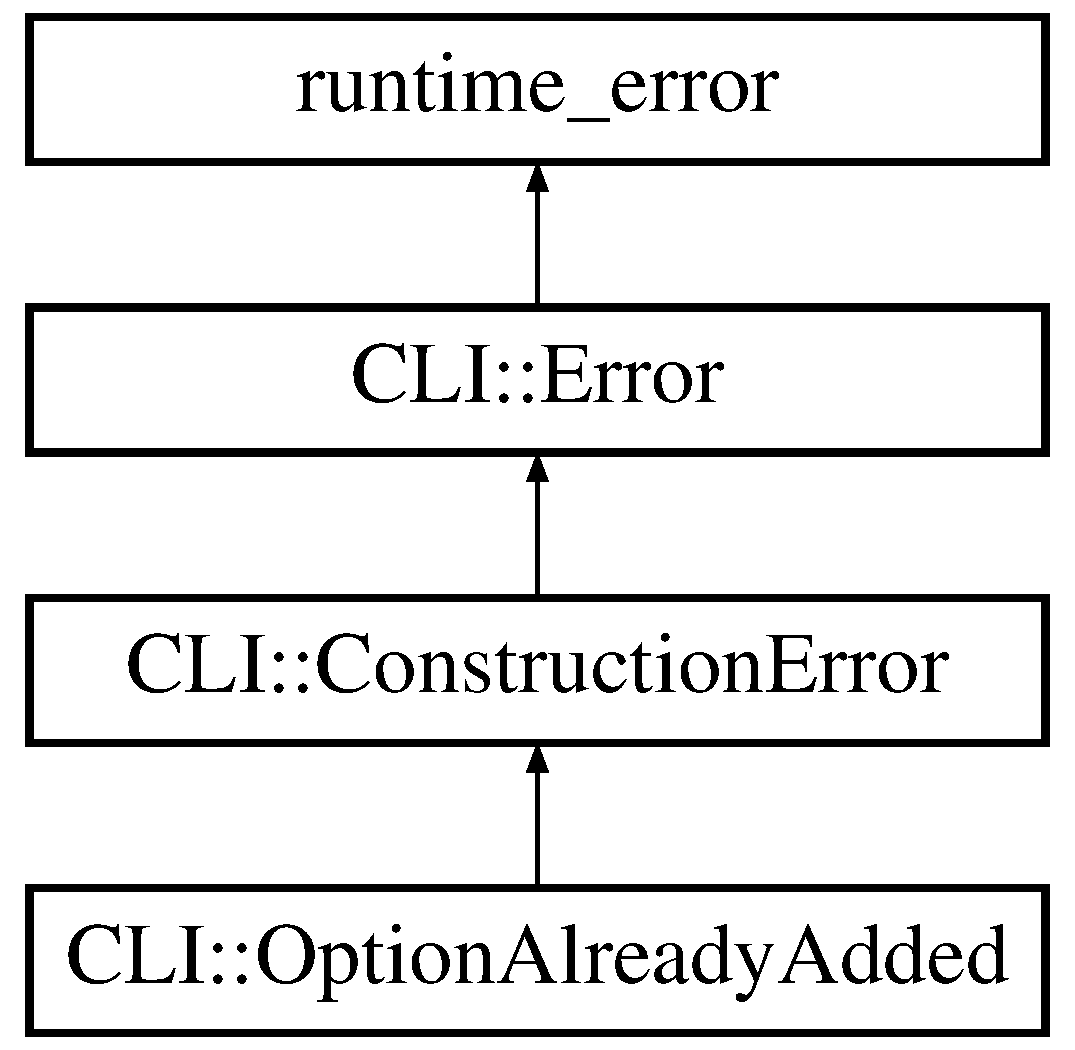
\includegraphics[height=4.000000cm]{struct_c_l_i_1_1_option_already_added}
\end{center}
\end{figure}
\subsection*{Public Member Functions}
\begin{DoxyCompactItemize}
\item 
\mbox{\Hypertarget{struct_c_l_i_1_1_option_already_added_a2157496f3b017fa4894fd4950206101c}\label{struct_c_l_i_1_1_option_already_added_a2157496f3b017fa4894fd4950206101c}} 
{\bfseries Option\+Already\+Added} (std\+::string name)
\end{DoxyCompactItemize}
\subsection*{Additional Inherited Members}


\subsection{Detailed Description}
Thrown when an option already exists. 

The documentation for this struct was generated from the following file\+:\begin{DoxyCompactItemize}
\item 
/home/travis/build/henryiii/\+C\+L\+I11/include/\+C\+L\+I/Error.\+hpp\end{DoxyCompactItemize}

\hypertarget{struct_c_l_i_1_1_option_not_found}{}\section{C\+LI\+:\+:Option\+Not\+Found Struct Reference}
\label{struct_c_l_i_1_1_option_not_found}\index{C\+L\+I\+::\+Option\+Not\+Found@{C\+L\+I\+::\+Option\+Not\+Found}}


Thrown when counting a non-\/existent option.  




{\ttfamily \#include $<$Error.\+hpp$>$}

Inheritance diagram for C\+LI\+:\+:Option\+Not\+Found\+:\begin{figure}[H]
\begin{center}
\leavevmode
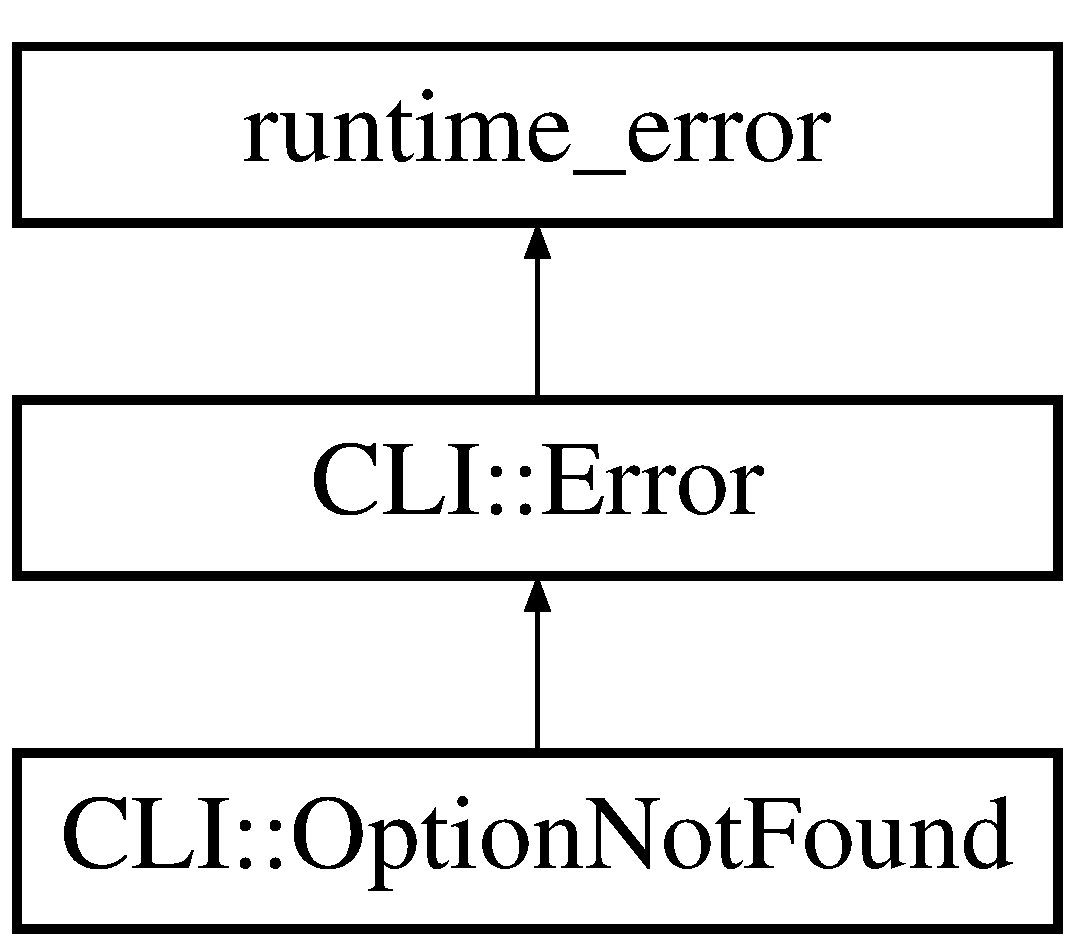
\includegraphics[height=3.000000cm]{struct_c_l_i_1_1_option_not_found}
\end{center}
\end{figure}
\subsection*{Public Member Functions}
\begin{DoxyCompactItemize}
\item 
\mbox{\Hypertarget{struct_c_l_i_1_1_option_not_found_a0abf448c748239711b5ed963f388ec1d}\label{struct_c_l_i_1_1_option_not_found_a0abf448c748239711b5ed963f388ec1d}} 
{\bfseries Option\+Not\+Found} (std\+::string name)
\end{DoxyCompactItemize}
\subsection*{Additional Inherited Members}


\subsection{Detailed Description}
Thrown when counting a non-\/existent option. 

The documentation for this struct was generated from the following file\+:\begin{DoxyCompactItemize}
\item 
/home/travis/build/henryiii/\+C\+L\+I11/include/\+C\+L\+I/Error.\+hpp\end{DoxyCompactItemize}

\hypertarget{struct_c_l_i_1_1_parse_error}{}\section{C\+LI\+:\+:Parse\+Error Struct Reference}
\label{struct_c_l_i_1_1_parse_error}\index{C\+L\+I\+::\+Parse\+Error@{C\+L\+I\+::\+Parse\+Error}}


Anything that can error in Parse.  




{\ttfamily \#include $<$Error.\+hpp$>$}

Inheritance diagram for C\+LI\+:\+:Parse\+Error\+:\begin{figure}[H]
\begin{center}
\leavevmode
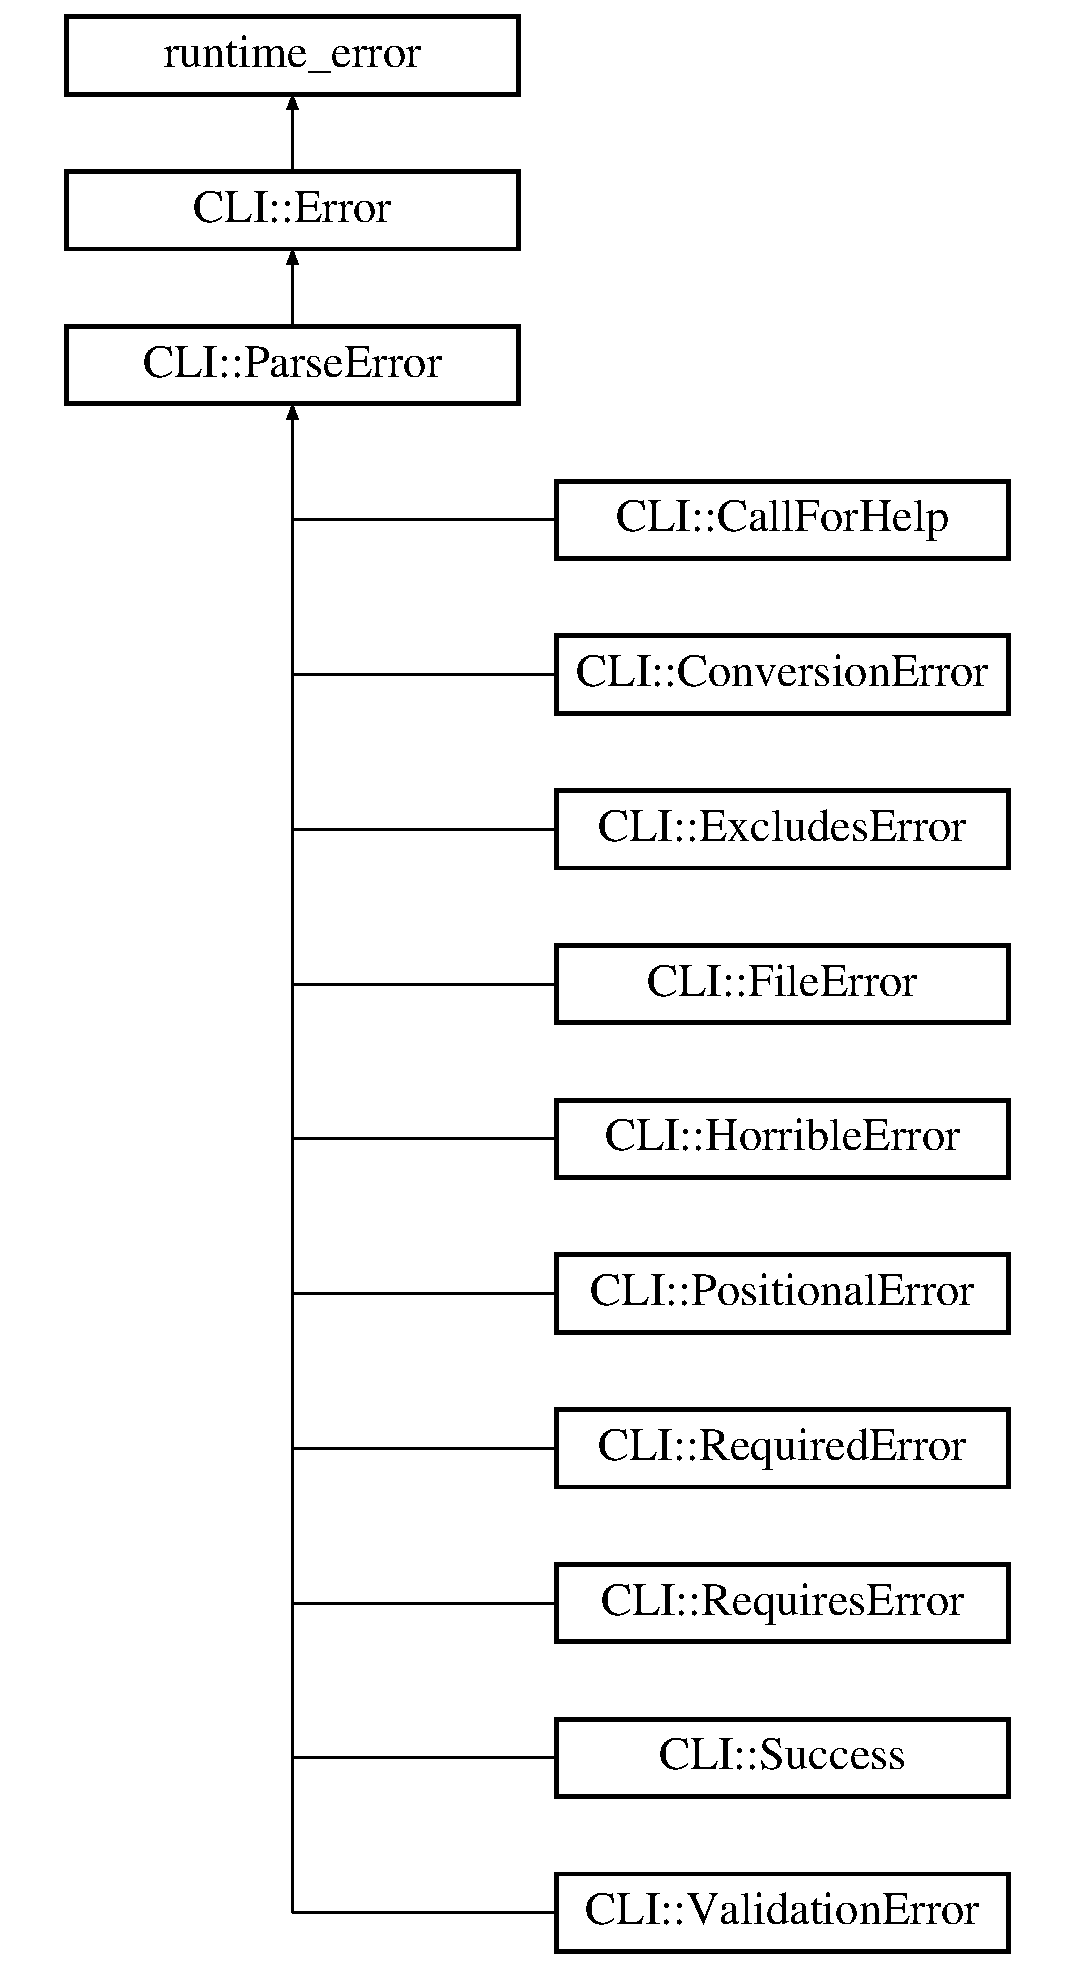
\includegraphics[height=12.000000cm]{struct_c_l_i_1_1_parse_error}
\end{center}
\end{figure}
\subsection*{Public Member Functions}
\begin{DoxyCompactItemize}
\item 
\mbox{\Hypertarget{struct_c_l_i_1_1_parse_error_ad7af7bf698b0fea17454b8cc27df19ab}\label{struct_c_l_i_1_1_parse_error_ad7af7bf698b0fea17454b8cc27df19ab}} 
{\bfseries Parse\+Error} (std\+::string parent, std\+::string name, int exit\+\_\+code=255, bool print\+\_\+help=true)
\end{DoxyCompactItemize}
\subsection*{Additional Inherited Members}


\subsection{Detailed Description}
Anything that can error in Parse. 

The documentation for this struct was generated from the following file\+:\begin{DoxyCompactItemize}
\item 
/home/travis/build/henryiii/\+C\+L\+I11/include/\+C\+L\+I/Error.\+hpp\end{DoxyCompactItemize}

\hypertarget{struct_c_l_i_1_1_positional_error}{}\section{C\+LI\+:\+:Positional\+Error Struct Reference}
\label{struct_c_l_i_1_1_positional_error}\index{C\+L\+I\+::\+Positional\+Error@{C\+L\+I\+::\+Positional\+Error}}


Thrown when too many positionals are found.  




{\ttfamily \#include $<$Error.\+hpp$>$}

Inheritance diagram for C\+LI\+:\+:Positional\+Error\+:\begin{figure}[H]
\begin{center}
\leavevmode
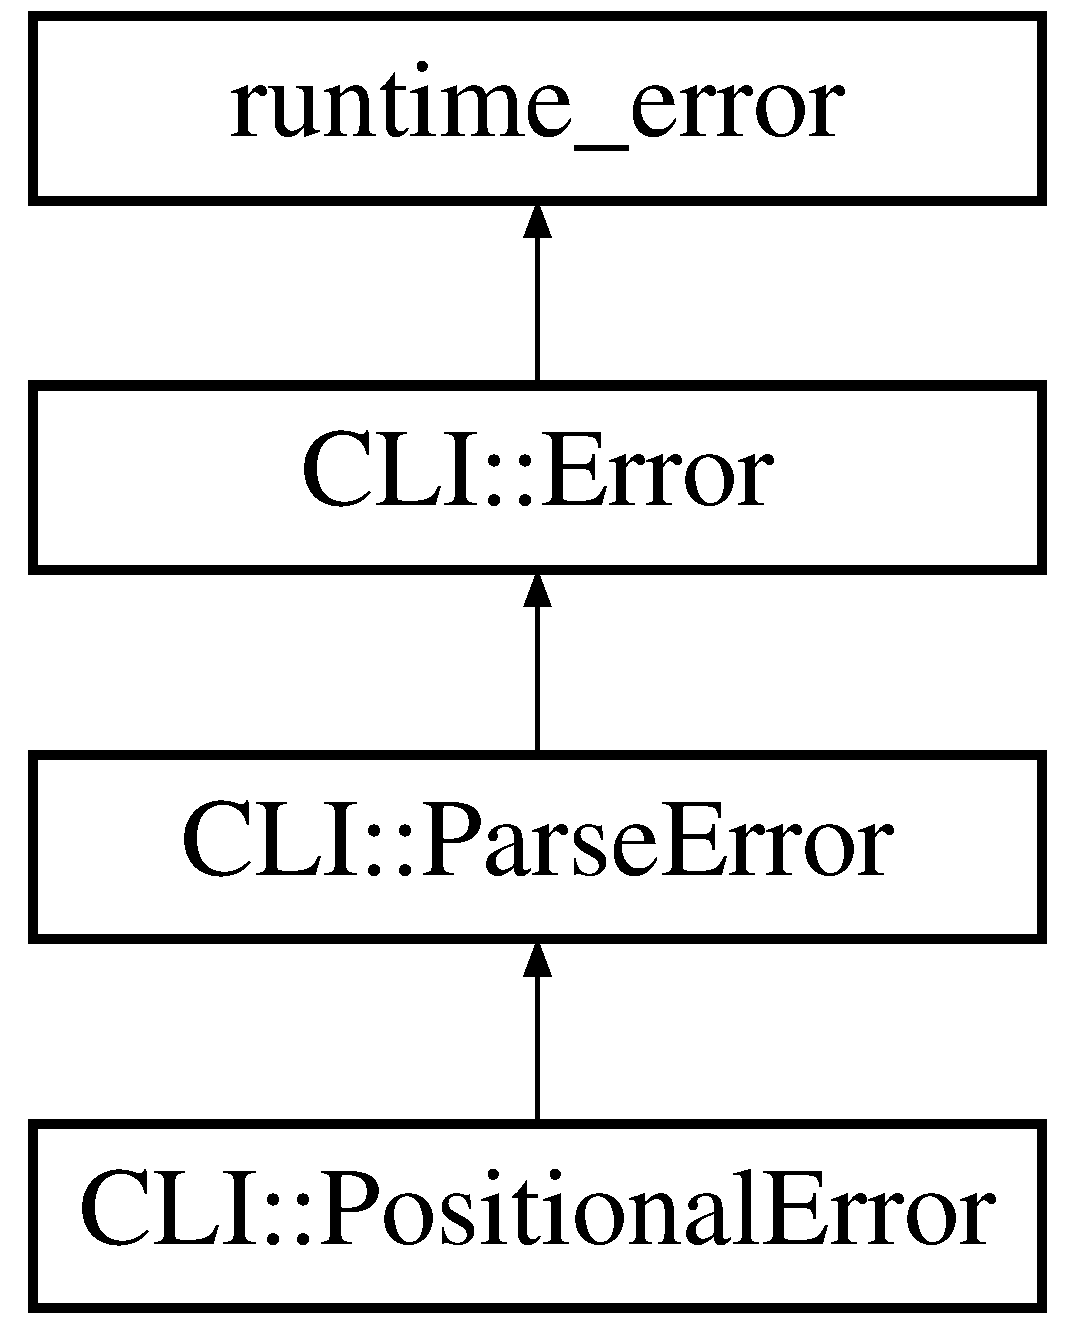
\includegraphics[height=4.000000cm]{struct_c_l_i_1_1_positional_error}
\end{center}
\end{figure}
\subsection*{Public Member Functions}
\begin{DoxyCompactItemize}
\item 
\mbox{\Hypertarget{struct_c_l_i_1_1_positional_error_acc0293ac28470702df76736c4beee449}\label{struct_c_l_i_1_1_positional_error_acc0293ac28470702df76736c4beee449}} 
{\bfseries Positional\+Error} (std\+::string name)
\end{DoxyCompactItemize}
\subsection*{Additional Inherited Members}


\subsection{Detailed Description}
Thrown when too many positionals are found. 

The documentation for this struct was generated from the following file\+:\begin{DoxyCompactItemize}
\item 
/home/travis/build/henryiii/\+C\+L\+I11/include/\+C\+L\+I/Error.\+hpp\end{DoxyCompactItemize}

\hypertarget{struct_c_l_i_1_1_required_error}{}\section{C\+LI\+:\+:Required\+Error Struct Reference}
\label{struct_c_l_i_1_1_required_error}\index{C\+L\+I\+::\+Required\+Error@{C\+L\+I\+::\+Required\+Error}}


Thrown when a required option is missing.  




{\ttfamily \#include $<$Error.\+hpp$>$}

Inheritance diagram for C\+LI\+:\+:Required\+Error\+:\begin{figure}[H]
\begin{center}
\leavevmode
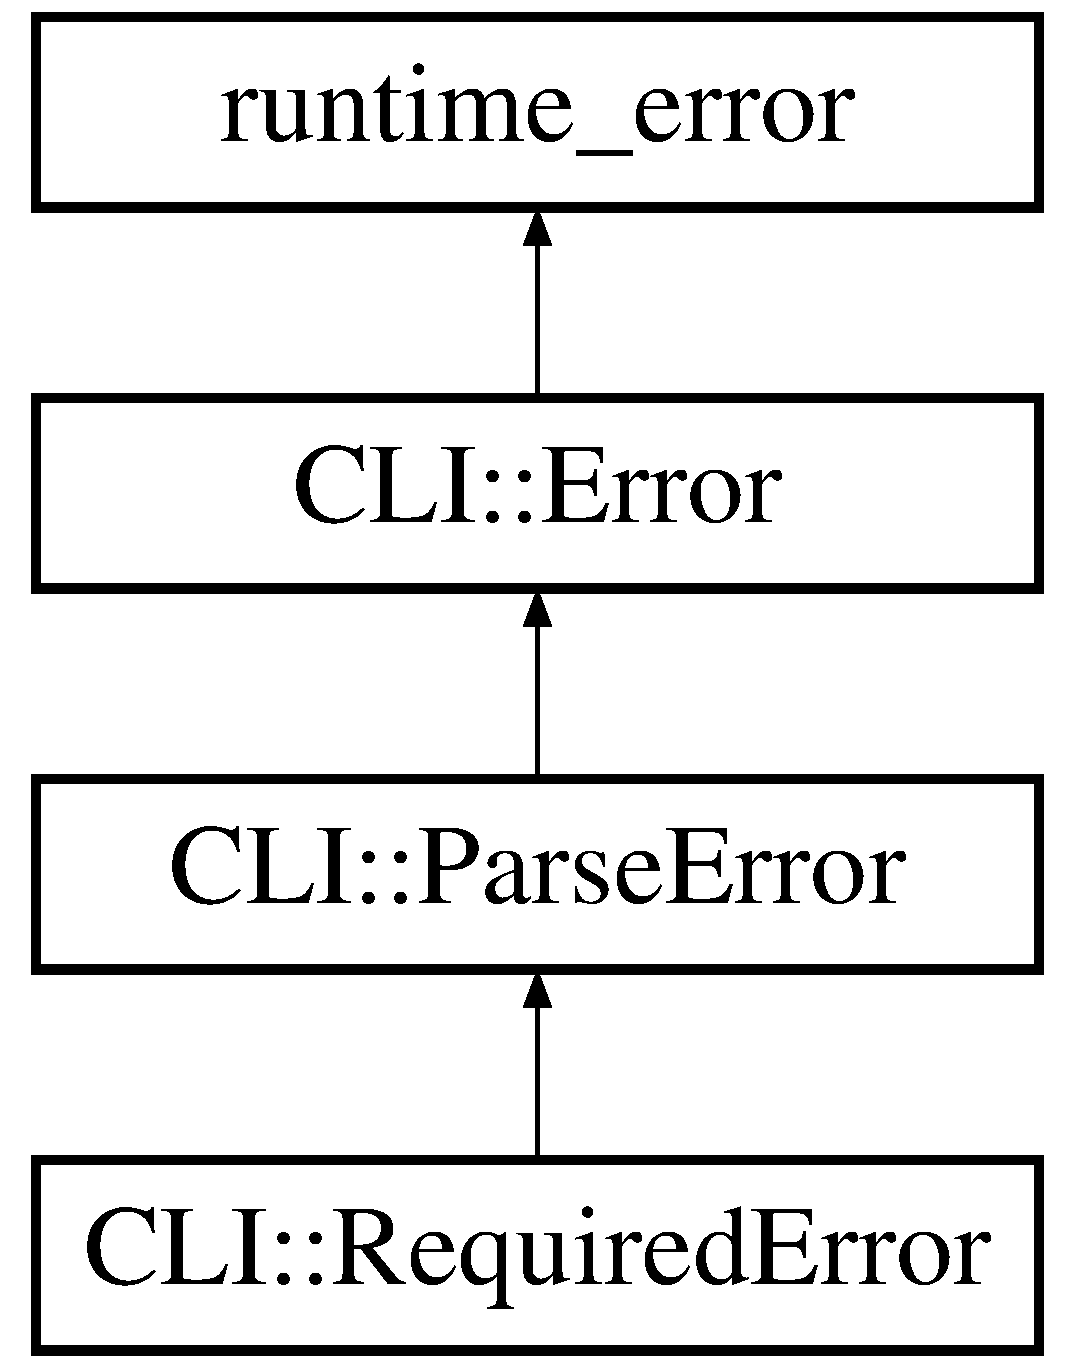
\includegraphics[height=4.000000cm]{struct_c_l_i_1_1_required_error}
\end{center}
\end{figure}
\subsection*{Public Member Functions}
\begin{DoxyCompactItemize}
\item 
\mbox{\Hypertarget{struct_c_l_i_1_1_required_error_a13150580687c3277d6d96cc0959c2adc}\label{struct_c_l_i_1_1_required_error_a13150580687c3277d6d96cc0959c2adc}} 
{\bfseries Required\+Error} (std\+::string name)
\end{DoxyCompactItemize}
\subsection*{Additional Inherited Members}


\subsection{Detailed Description}
Thrown when a required option is missing. 

The documentation for this struct was generated from the following file\+:\begin{DoxyCompactItemize}
\item 
/home/travis/build/henryiii/\+C\+L\+I11/include/\+C\+L\+I/Error.\+hpp\end{DoxyCompactItemize}

\hypertarget{struct_c_l_i_1_1_requires_error}{}\section{C\+LI\+:\+:Requires\+Error Struct Reference}
\label{struct_c_l_i_1_1_requires_error}\index{C\+L\+I\+::\+Requires\+Error@{C\+L\+I\+::\+Requires\+Error}}


Thrown when a requires option is missing.  




{\ttfamily \#include $<$Error.\+hpp$>$}

Inheritance diagram for C\+LI\+:\+:Requires\+Error\+:\begin{figure}[H]
\begin{center}
\leavevmode
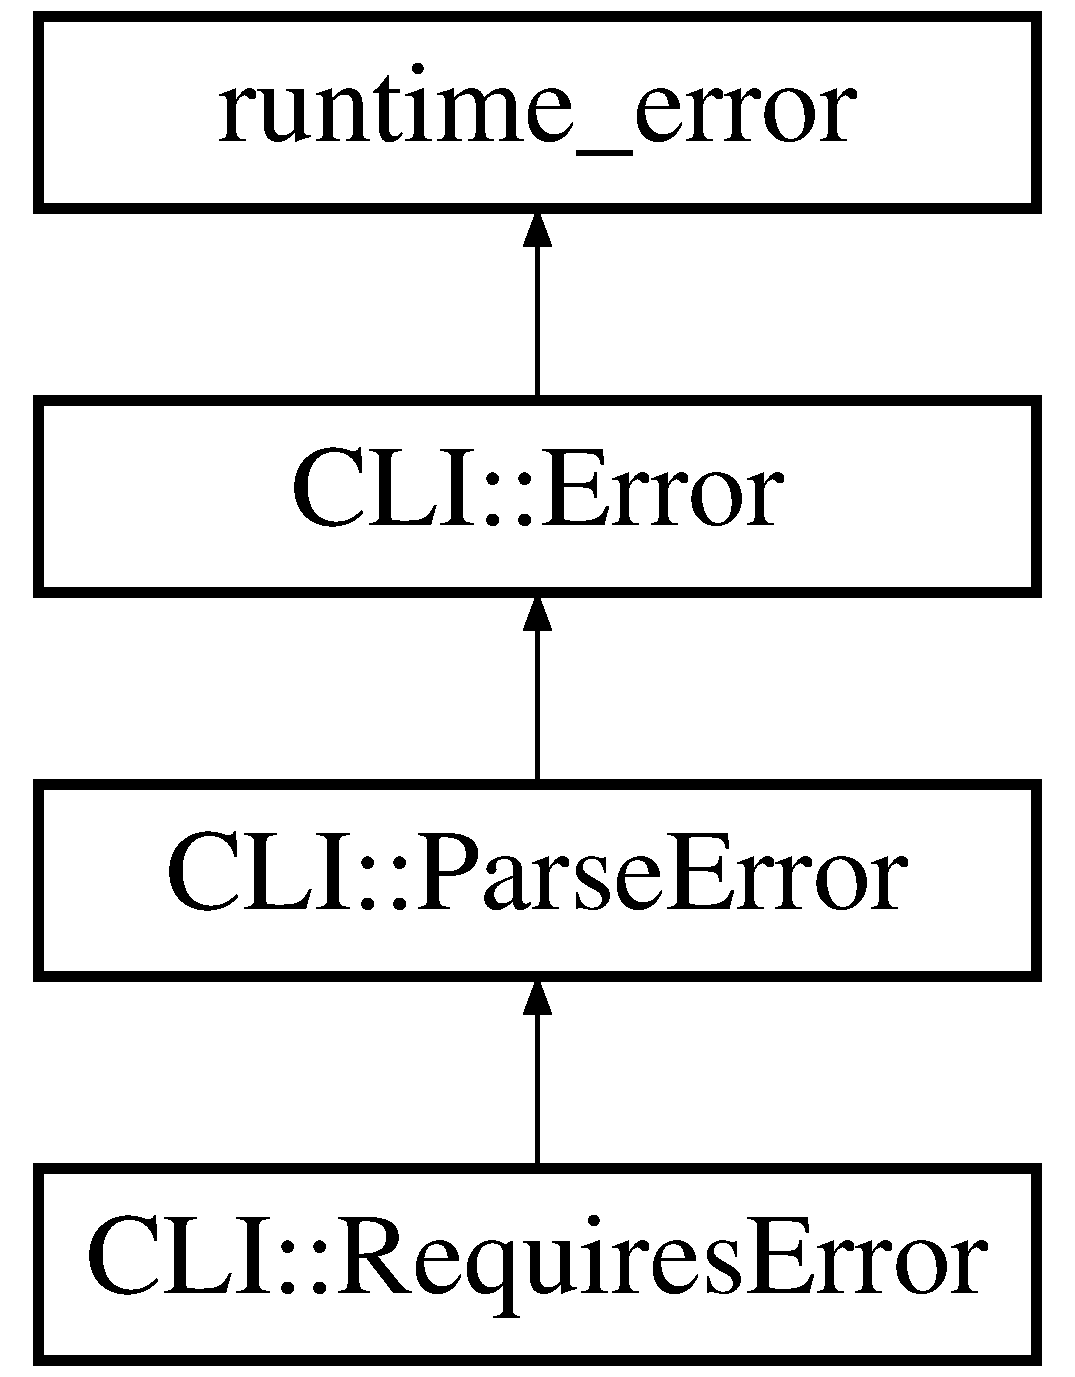
\includegraphics[height=4.000000cm]{struct_c_l_i_1_1_requires_error}
\end{center}
\end{figure}
\subsection*{Public Member Functions}
\begin{DoxyCompactItemize}
\item 
\mbox{\Hypertarget{struct_c_l_i_1_1_requires_error_afb74d006a67ea1e3ef2a3a400d64517b}\label{struct_c_l_i_1_1_requires_error_afb74d006a67ea1e3ef2a3a400d64517b}} 
{\bfseries Requires\+Error} (std\+::string name, std\+::string subname)
\end{DoxyCompactItemize}
\subsection*{Additional Inherited Members}


\subsection{Detailed Description}
Thrown when a requires option is missing. 

The documentation for this struct was generated from the following file\+:\begin{DoxyCompactItemize}
\item 
/home/travis/build/henryiii/\+C\+L\+I11/include/\+C\+L\+I/Error.\+hpp\end{DoxyCompactItemize}

\hypertarget{struct_c_l_i_1_1_success}{}\section{C\+LI\+:\+:Success Struct Reference}
\label{struct_c_l_i_1_1_success}\index{C\+L\+I\+::\+Success@{C\+L\+I\+::\+Success}}


This is a successful completion on parsing, supposed to exit.  




{\ttfamily \#include $<$Error.\+hpp$>$}

Inheritance diagram for C\+LI\+:\+:Success\+:\begin{figure}[H]
\begin{center}
\leavevmode
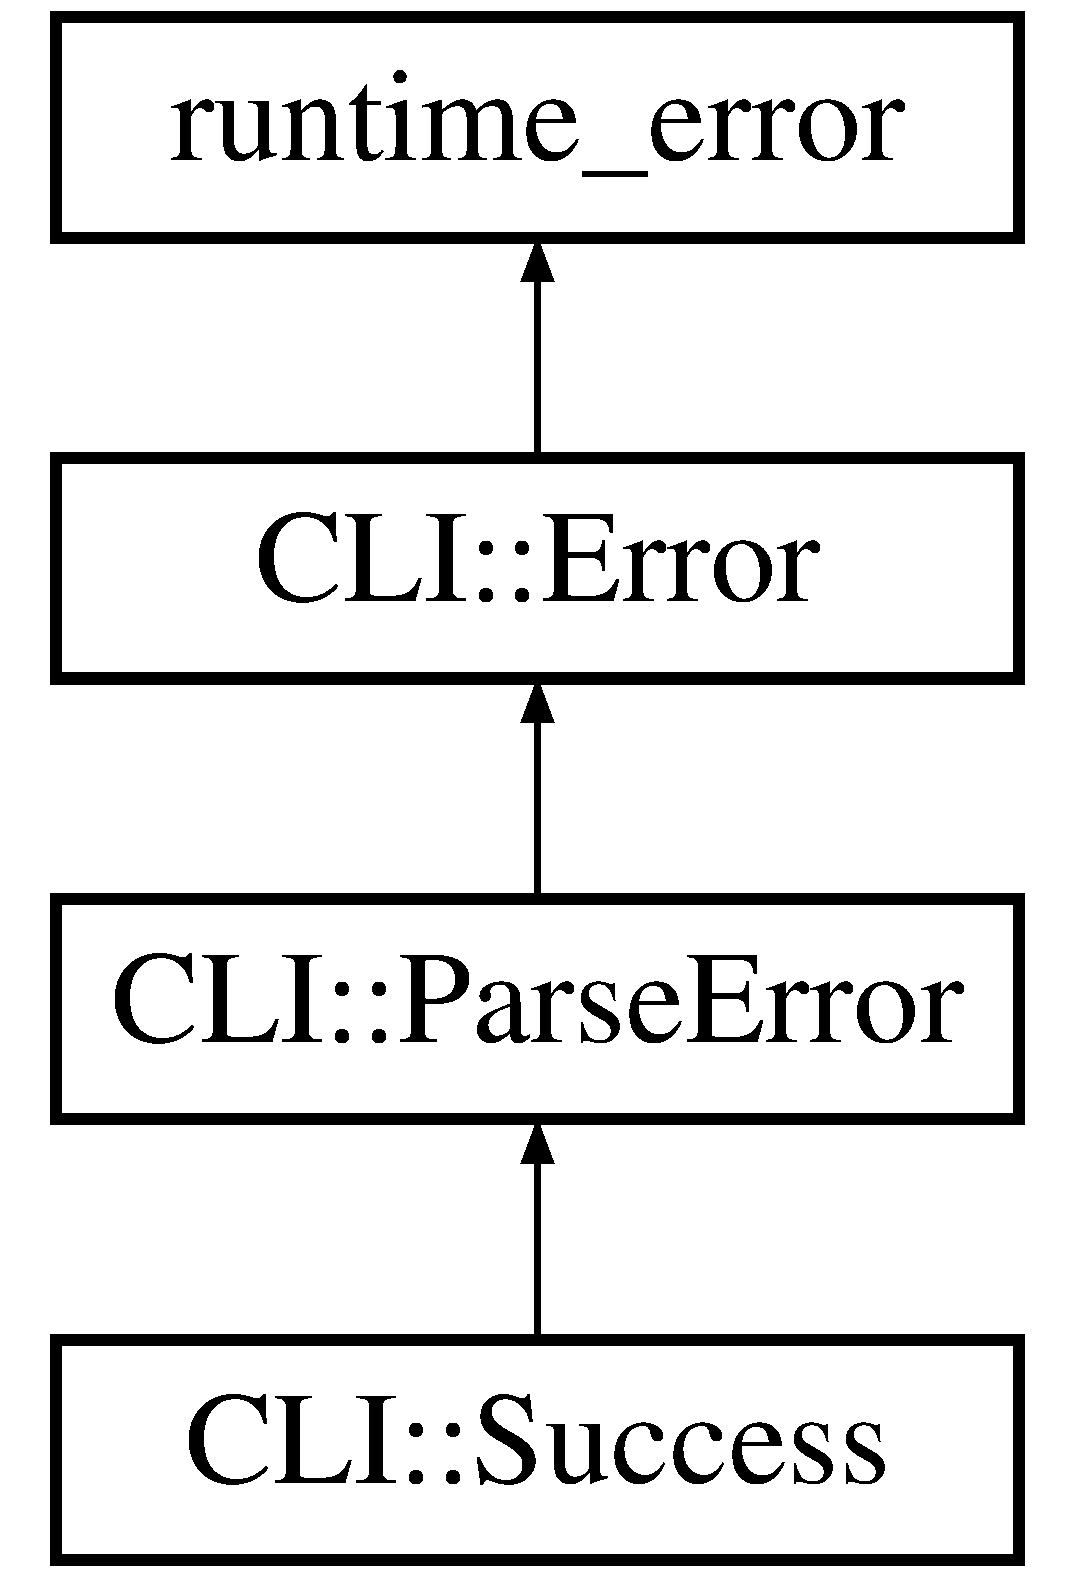
\includegraphics[height=4.000000cm]{struct_c_l_i_1_1_success}
\end{center}
\end{figure}
\subsection*{Additional Inherited Members}


\subsection{Detailed Description}
This is a successful completion on parsing, supposed to exit. 

The documentation for this struct was generated from the following file\+:\begin{DoxyCompactItemize}
\item 
/home/travis/build/henryiii/\+C\+L\+I11/include/\+C\+L\+I/Error.\+hpp\end{DoxyCompactItemize}

\hypertarget{struct_c_l_i_1_1_validation_error}{}\section{C\+LI\+:\+:Validation\+Error Struct Reference}
\label{struct_c_l_i_1_1_validation_error}\index{C\+L\+I\+::\+Validation\+Error@{C\+L\+I\+::\+Validation\+Error}}


Thrown when validation of results fails.  




{\ttfamily \#include $<$Error.\+hpp$>$}

Inheritance diagram for C\+LI\+:\+:Validation\+Error\+:\begin{figure}[H]
\begin{center}
\leavevmode
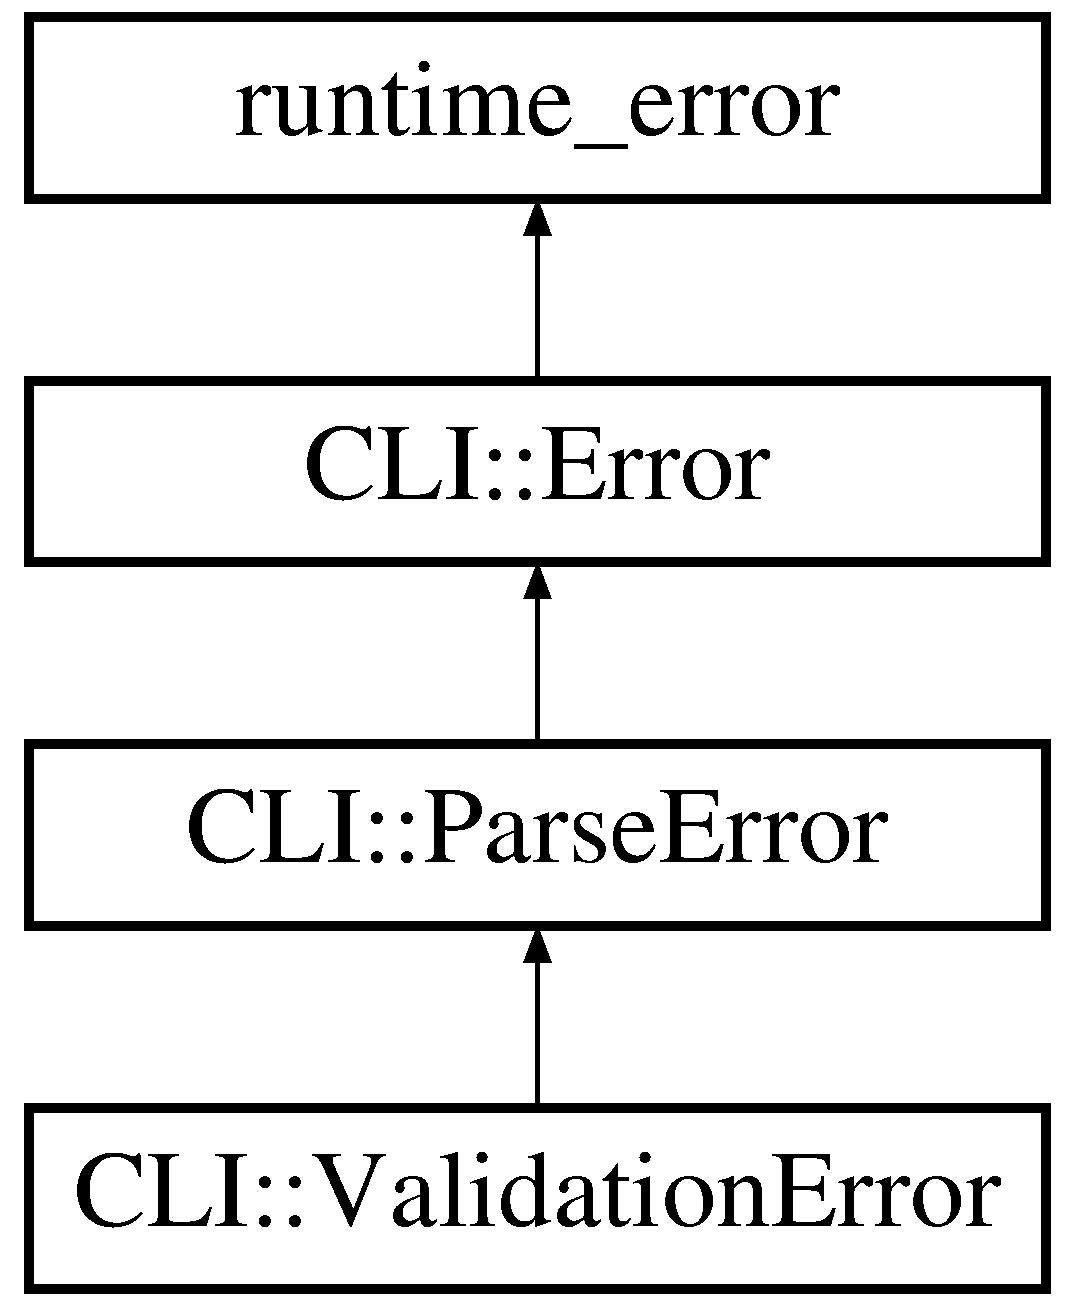
\includegraphics[height=4.000000cm]{struct_c_l_i_1_1_validation_error}
\end{center}
\end{figure}
\subsection*{Public Member Functions}
\begin{DoxyCompactItemize}
\item 
\mbox{\Hypertarget{struct_c_l_i_1_1_validation_error_ae1e2233b5668b07af2c96b9ff7d02a5a}\label{struct_c_l_i_1_1_validation_error_ae1e2233b5668b07af2c96b9ff7d02a5a}} 
{\bfseries Validation\+Error} (std\+::string name)
\end{DoxyCompactItemize}
\subsection*{Additional Inherited Members}


\subsection{Detailed Description}
Thrown when validation of results fails. 

The documentation for this struct was generated from the following file\+:\begin{DoxyCompactItemize}
\item 
/home/travis/build/henryiii/\+C\+L\+I11/include/\+C\+L\+I/Error.\+hpp\end{DoxyCompactItemize}

%--- End generated contents ---

% Index
\backmatter
\newpage
\phantomsection
\clearemptydoublepage
\addcontentsline{toc}{chapter}{Index}
\printindex

\end{document}
